\documentclass[12pt,a4paper]{scrartcl}
\usepackage{forest}
\usepackage{booktabs}
\usepackage{nameref}
\usepackage[breaklinks=true]{hyperref}
\usepackage{placeins}
\usepackage{titling}
\usepackage{graphicx}
\usepackage{listings}

\graphicspath{{figures/}{../figures/}}
\renewcommand{\subtitle}[1]{%
  \posttitle{%
    \par\end{center}
    \begin{center}\large#1\end{center}
    \vskip0.5em}%
}
\title{Laminar EEG-fMRI pipeline}
\author{Tommy Clausner}
\subtitle{\textsc{Documentation}}
\date{\small{last updated on \today}}

\begin{document}
\setcounter{secnumdepth}{1}
\begin{titlepage}
\clearpage\maketitle
\thispagestyle{empty}
\end{titlepage}
\tableofcontents
\newpage
\section{About this Document}
\label{sec:about}
This documententation accompanies the scripts that I wrote for my MSc thesis on feature specific neuronal oscillations on a cortical laminar level under the supervision of:
\begin{itemize}
  \item Mathilde Bonnefond
  \item Rene Scheeringa
\end{itemize}
Hence all the functionality is tied to our specific experiment. However, most steps still can serve as a template for laminar EEG-fMRI analyses in general.\\
\noindent Our experiment consisted of 3 major parts: retinotopic field mapping for visual ROI definition, odd ball task employing gabbor patches (main task) and additional support scans as there are: T1 anatomical and functional scans with inversed flip angle. During the main task EEG was recorded in a $3~s$ gap between blocks of $3~TR$ (3 functional volumes). This led to a signal drop off over each of the third fMRI volumes, that was absent during retinotopy scans. We exploited the fact that the difference between the 3rd and 1st volume of such a block yields a T1-like contrast, to optimise co-registration performance.\\
\noindent To enable myself to write all the scripts I got help from various people, so further thanks goes to:
\begin{itemize}
  \item Jose Marques
  \item Koen Haak
  \item Matthias Ekman
  \item Simon Hom\"olle
  \item Tim van Mourik
  \item TG guys at the DCCN
\end{itemize}
The goal was to create a set of scripts such that it would be highly standardized and with as little human interaction as possible. This way it is guaranteed, that once the analysis and respective parameters are set up, the scripts will run similar for all subjects. However it also means that changing single scripts within this "ecosystem" should be done very carefully to not interfere with relative paths and file I/O all functions rely on.
\section{Before starting}
Most of the functionality is optimized for the IT infrastructure provided by the Donders Center for Cognitive Neuroimaging. Since some parts of the analysis require very high amounts of memory, those parts are absolutely infeasible to compute on a local desktop or laptop machine. Given the infrastructure of the DCCN, all scripts were optimized to a reasonable amount for a reduction in computation time but still keeping high spatial accuracy. Hence parts might need to be adjusted to either a different cluster computing system or scaled down massively.\\
All scripts as we used them can be found at \href{https://github.com/TommyClausner/laminarfMRI}{\nolinkurl{https://github.com/TommyClausner/laminarfMRI}}
or by cloning the GitHub repository via the command line:
\begin{lstlisting}[
    language=Shell,
    basicstyle=\ttfamily,
    breaklines=true]
    # download scripts
    git clone https://github.com/TommyClausner/laminarfMRI
\end{lstlisting}
\subsection{Pre- requisites}
\label{sec:prereq}
The present pipeline makes use of many modern state of the art analysis toolboxes for Shell and or MATLAB scripting:
\begin{itemize}
\item analysePRF (\href{http://kendrickkay.net/analyzePRF/}{\nolinkurl{http://kendrickkay.net/analyzePRF/}})
\item FieldTrip (\href{https://github.com/fieldtrip/fieldtrip}{\nolinkurl{https://github.com/fieldtrip/fieldtrip}})
\item FreeSurfer (\href{https://surfer.nmr.mgh.harvard.edu/}{\nolinkurl{https://surfer.nmr.mgh.harvard.edu/}})
\item FSL (\href{https://fsl.fmrib.ox.ac.uk/fsl/fslwiki}{\nolinkurl{https://fsl.fmrib.ox.ac.uk/fsl/fslwiki}})
\item knkutils (\href {https://github.com/kendrickkay/knkutils/}{\nolinkurl{https://github.com/kendrickkay/knkutils/}})
\item MATLAB R2015a or later (\href{https://nl.mathworks.com/products/matlab.html}{\nolinkurl{https://nl.mathworks.com/products/matlab.html}})
\item MRIcron (\href{https://www.nitrc.org/projects/mricron}{\nolinkurl{https://www.nitrc.org/projects/mricron}})
\item Open fMRI Analysis (\href{https://github.com/TimVanMourik/OpenFmriAnalysis}{\nolinkurl{https://github.com/TimVanMourik/OpenFmriAnalysis}})
\item Pipeline (\href{https://github.com/Washington-University/Pipeline}{\nolinkurl{https://github.com/Washington-University/Pipeline}})
\item PsychToolbox (\href{https://github.com/Psychtoolbox-3/Psychtoolbox-3}{\nolinkurl{https://github.com/Psychtoolbox-3/Psychtoolbox-3}})
\item SPM (\href{http://www.fil.ion.ucl.ac.uk/spm/}{\nolinkurl{http://www.fil.ion.ucl.ac.uk/spm/}})
\item tc\_functions  (\href{https://github.com/TommyClausner/tc\_functions}{\nolinkurl{https://github.com/TommyClausner/tc\_functions}})
\item VistaSoft (\href{https://github.com/vistalab/vistasoft}{\nolinkurl{https://github.com/vistalab/vistasoft}})
\item Workbench (\href{https://github.com/Washington-University/Workbench}{\nolinkurl{https://github.com/Washington-University/Workbench}})
\end{itemize}

\noindent Use e.g. MRIcron's dicom2nii to convert raw MRI data to NIfTI files.\\

\noindent Call the function \texttt{\nameref{sh:getTools}} to download (most of) the software automatically into a folder called toolboxes/ located in the folder from where the function was called (see \texttt{\nameref{sh:getTools}} and Figure~\ref{tree:folderstruct})\\
\begin{lstlisting}[
    language=Shell,
    basicstyle=\ttfamily,
    breaklines=true]
    # download toolboxes
    sh getToolboxes.sh
\end{lstlisting}

\subsection{Folder structure}
\label{sec:dirstruct}
The general folder structure is set up by a call to setupfolders.sh (see also Figure \ref{tree:folderstruct}). Raw data should be placed in the corresponding subfolder:
\begin{itemize}
\item Functional data must be located in rawData/niftis/\textbf{functionals}/
\item Anatomical data must be located in in rawData/niftis/\textbf{t1}/
\item Inverted functional data must be located in in rawData/niftis/\textbf{inverted}/
\item Proton density data must be located in in rawData/niftis/\textbf{wholeBrainEPI3D}/
\item Inverted proton density data must be located in in rawData/niftis/\textbf{wholeBrainEPI3Dinverted}/
\item EEG data must be located in rawData/\textbf{eegfiles}/
\item Eye tracking data must be located in rawData/\textbf{eyetrackerfiles}/
\item EEG sensor position related files must be in rawData/\textbf{electrodes}/
\item electromagnetic digitizer data must be in rawData/electrodes/\textbf{polhemus}/
\item photogrammetry data must be in rawData/electrodes/\textbf{photogrammetry}/ (note also the respective sub-structure, set up by \texttt{\nameref{sh:setDir}})
\end{itemize}

\subsection{How things work}
\noindent\textbf{Bash scripts}\\
\noindent Parts of the analysis run in Bash scripts. Those should be called from their root directory using:
\begin{lstlisting}[
    language=Shell,
    basicstyle=\ttfamily,
    breaklines=true]
    # run scripts
    sh scriptname.sh
\end{lstlisting}
Each step within the analysis has a different subfolder containing the respective results of this step. Leading numbers indicate in which logical order the corresponding shell scripts should be executed. Note that all files created by each respective step are stored in the corresponding folder. However files that need to be preset (e.g. config files) must be located in A\_helperfiles.\\

\noindent\textbf{MATLAB wrapper}\\
\noindent Note, that most EEG related scripts rely on MATLAB and FieldTrip. Those scripts can be run stand-alone inside MATLAB or using the bash-script wrapper that has the exact same name only with the file extension \texttt{.sh} instead of \texttt{.m} Furthermore some MATLAB scipts require significant computation time, for which reason they are set up to be run as parts of a whole. In this case the words \textit{split} is added to the file name. Those scripts call the corresponding shell scripts that call the MATLAB scripts in turn, in a organized manner to be run on the cluster.\\

\noindent When using such a MATLAB wrapper some MATLAB language specific details and variables are added to the base-file (\texttt{targetScript.m}). In every case the respective absolute folder path is provided. The shell script creates a temporary file and run it. It will be constructed by adding variables to an empty file and afterwards adding the actual base-file like so:
\begin{lstlisting}[
    language=Shell,
    basicstyle=\ttfamily,
    breaklines=true]
    # guts of MATLAB wrapper
    DIR="$( cd "$( dirname "${BASH_SOURCE[0]}" )" && pwd )"
    cd $DIR
    nameadd=$(date +"%m%d%Y%H%M%S")
    echo "mainpath=" "'$DIR';">$DIR/tmp_$nameadd.m
    cat $DIR/targetScript.m>>$DIR/tmp_$nameadd.m
    echo 'matlab2017b -nosplash -r "run('"'"$DIR/tmp_$nameadd.m"'"');"'  | qsub -q $jobtype -l walltime=$walltime,mem=$memory
\end{lstlisting}
\medskip
\noindent\textbf{a note on EEG}\\
\noindent Files processing EEG data will have the prefix \texttt{do\_EEG} and have a in itself closed workflow. This is mostly due to the fact, that scripts merely run in MATLAB at some point.\\
\noindent To keep the data somewhat structured, a new datafile is created after each major processing step, adding a new prefix to the file name. E.g. after the time-frequency analysis \texttt{TF\_} will be added to the current file name making \texttt{my\_data.mat} becoming \texttt{TF\_my\_data.mat}\\

\noindent Within each function it can be defined, which is the prefix of the data to load and which is the prefix that will be added after results were computed. The default will be stated in the respective detailed explaination in Section~\ref{sec:scriptsExplained}. However, after running \texttt{\nameref{m:selchan}} all in that file defined prefixes that are found in the EEG folder will be deleted, keeping only essential files like headmodel, sourcemodel, sensors and the results file.\\

\subsection{Helper files}
There are several helper files that are needed in order to perform the analysis:\\

\noindent\textbf{acquisition\_parameters.txt}

\noindent indicating the respective acquisition parameters per volume needed in order to perform the distortion correction. One line indicates the respective parameter setting for the respective volume (1st line corresponds to 1st volume, etc.)\\

\noindent e.g.:

\noindent 0 1 0 0.042\\
\noindent 0 -1 0 0.042\\

The first 3 columns indicate the respective phase coding direction the last column some weird value, that is only important if it changes. Otherwise it's fine to use any value as long as it is the same.\\

\noindent\textbf{b02b0.cnf}

\noindent Settings for distortion correction.

Needed in order to set the parameters for the distortion correction (example provided by FSL). For more information see \href{https://fsl.fmrib.ox.ac.uk/fsl/fslwiki/topup/TopupUsersGuide/}{\nolinkurl{https://fsl.fmrib.ox.ac.uk/fsl/fslwiki/topup/TopupUsersGuide/}}.\\

\noindent\textbf{params.mat}

\noindent Parameters used for retinotopy scans as obtained from VistaDisp. For more information see \href{https://web.stanford.edu/group/vista/cgi-bin/wiki/index.php/Stimulus}{\nolinkurl{https://web.stanford.edu/group/vista/cgi-bin/wiki/index.php/Stimulus}}.\\

\noindent\textbf{images.mat}

\noindent Stimuli used for retinotopy scans. Stimuli file must be such that each frame is represented as a binary image. The matrix must be of shape $Y \times X \times T$ where $X$ and $Y$ are the image dimensions in pixel and T is the respective number of frames.

\subsection{qsub}
Scripts that are flagged with the (Q) can be submitted as a qsub job.

\noindent When running the computation on the cluster use the wrapper function runonqsub.sh like so
\begin{lstlisting}[
    language=Shell,
    basicstyle=\ttfamily,
    breaklines=true]
    # run scripts on cluster using wrapper function
    sh runonqsub.sh 32gb targetScript.sh
\end{lstlisting}


\noindent Note that some scripts send a MATLAB script to the qsub cluster. Thus they cannot be run using \texttt{\nameref{sh:runQsub}}, but instead create their own job. However those scripts can also run stand-alone within a interactive MATLAB session.\\

\noindent Table~\ref{tab:hardwarerequirements} gives an overview about requirements on memory and computation time can be expected:

\begin{table}[h]
\centering
\begin{tabular}{l | r | l}
\toprule
script & memory required & time required\\\hline
  \nameref{sh:combsplt} & 64GB & $\approx 10min$ \\\hline
  \nameref{sh:analyzePRF} & 6GB & $\approx 4-10h$ \\\hline
  \nameref{sh:applydistcorr} & 32GB & $\approx 30min$ \\\hline
  \nameref{sh:coreg} & 16GB & $\approx 30min$ \\\hline
  \nameref{sh:corravg} & 4GB & $\approx 3sec$ \\\hline
  \nameref{sh:distcorr} & 32GB & $\approx 15min$ \\\hline
  \nameref{sh:beamf} & 60GB & $\approx 5h$ \\\hline
  \nameref{sh:selchan} & 256GB & $\approx 30min$ \\\hline
  \nameref{sh:freqVirt} & 60GB & $\approx 5h$ \\\hline
  \nameref{sh:prepFS4EEG} & 8GB & $\approx 10min$ \\\hline
  \nameref{sh:prepHM} & 32GB & $\approx 10min$ \\\hline
  \nameref{sh:prepSM} & 32GB & $\approx 6-8h$ \\\hline
  \nameref{sh:EEGpreproc} & 16GB & $\approx 30min$ \\\hline
  \nameref{sh:splitbeamf} & 480GB & $\approx 5h$ \\\hline
  \nameref{sh:splitfreqVirt} & 960GB & $\approx 5h$ \\\hline
  \nameref{sh:splitvirtch} & 240GB & $\approx 5h$ \\\hline
  \nameref{sh:timelock} & 16GB & $\approx 5min$ \\\hline
  \nameref{sh:virtch} & 30GB & $\approx 5h$ \\\hline
  \nameref{sh:fsrecon} & 16GB & $\approx 6h$ \\\hline
  \nameref{sh:getLyr} & 16GB & $\approx 20min$ \\\hline
  \nameref{sh:getLyrW} & 16GB & $\approx 5min$ \\\hline
  \nameref{sh:msklbl} & 16GB & $\approx 1min$ \\\hline
  \nameref{sh:prepcoreg} & 16GB & $\approx 4.5h$ \\\hline
  \nameref{sh:prepfct} & 32GB & $\approx 10min$ \\\hline
  \nameref{sh:realign} & 32GB & $\approx 30min$ \\\hline
  \nameref{sh:splitanalyzePRF} & 480GB & $\approx 4-10h$ \\\hline
  \nameref{sh:tseriesinterp} & 64GB & $\approx 20min$ \\\hline
  \nameref{sh:GUI2ROI} & 8GB & user dependent \\\hline
  \nameref{sh:lbl2msk} & 8GB & $\approx 10s$ \\\hline
  \nameref{sh:mkOver} & 16GB & $\approx 5min$\\\hline
  \nameref{sh:mkprfO} & 16GB & $\approx 10min$ \\\bottomrule
\end{tabular}
\caption[Approximated time and memory requirements when running on qsub]{Approximated time and memory requirements for the respective script to run. Note that everything that is more than 4GB should be run on the cluster. Use runonqsub.sh or the respective MATLAB wrapper for that purpose.}
\label{tab:hardwarerequirements}
\end{table}

\newpage
\begin{figure}
\caption{Initial folder structure as required for the analysis}
\vspace{10pt}
{\scriptsize
\begin{forest}
  for tree={
    font=\ttfamily,
    grow'=0,
    child anchor=west,
    text height=0.01cm,
    parent anchor=south,
    anchor=west,
    calign=first,
    edge path={
      \noexpand\path [draw, \forestoption{edge}]
      (!u.south west) +(12pt,0pt) |- node[fill,inner sep=1.25pt] {} (.child anchor)\forestoption{edge label};
    },
    before typesetting nodes={
      if n=1
        {insert before={[,phantom]}}
        {}
    },
    fit=band,
    before computing xy={l=20pt},
  }
  [Analysis folder
[toolboxes/
    [see Section \ref{sec:prereq}]
  ]
[S\#/ (set up by setupfolders.sh or when created using makenewsubject.sh)
  [0\_freesurfer/
  ]
  [1\_realignment/
  ]
  [2\_distcorrection/
  ]
  [3\_coregistration/
  ]
  [4\_retinotopy/
  ]
  [5\_laminar/
  ]
  [6\_EEG/
  ]
  [7\_results/
  ]
  [A\_helperfiles/
    [acquisition\_parameters.txt]
    [b02b0.cnf]
    [params.mat]
    [images.mat]
  ]
  [B\_scripts/
    [*.m]
    [*.pipe]
    [*.sh]
  ]
  [C\_miscResults/
  ]
    [rawData/
      [niftis/
      [functionals/]
      [inverted/]
      [wholeBrainEPI3D/]
      [wholeBrainEPI3Dinverted/]
      [t1/]
      ]
      [eegfiles/]
      [electrodes/
        [photogrammetry/
          [3Dobject/]
          [photographs/
            [masks/]
          ]
          [photoscanfiles/]
        ]
        [polhemus/]
      ]
      [eyetrackerfiles/]
      [retinotopy/]
    ]
]
[template\_session/
[template\_helperfiles/
	[acquisition\_parameters.txt]
  [b02b0.cnf]
  [b02b0\_example\_fsl.cnf]
  [params.mat]
  [images.mat]
]
[template\_scripts/
	[*.m]
  [*.pipe]
  [*.sh]
]
]
[makenewsubject.sh]
[getToolboxes.sh]
]
\end{forest}

}
\label{tree:folderstruct}
\end{figure}

\FloatBarrier

\section{Quick Start}
This document builds upon the analysis rational used during our own analyses. It is build upon the technically facilities of the DCCN (Radboud University Nijmegen, 2018). Hence a copy-paste workflow will only work on a very similar infrastructure.\\
\subsection{first steps}
\begin{table}[h]
%\centering
\begin{tabular}{l | r}
\toprule
maximum memory required & approx time required\\\toprule
32GB & $\approx 10min+user$ \\\bottomrule
\end{tabular}
\end{table}
\FloatBarrier
\noindent Since you are reading this document, it is unlikely that you haven't done already, but the first step would be to download the required scripts by cloning or downloading the GitHub repository:
\begin{lstlisting}[
    language=Shell,
    basicstyle=\ttfamily,
    breaklines=true]
    # download scripts and toolboxes
    cd myPath
    git clone https://github.com/TommyClausner/laminarfMRI
    cd laminarfMRI/quickStart
    sh getToolboxes.sh
\end{lstlisting}
Figure~\ref{tree:folderstruct} depicts an overview of how the analysis folder should look like. Individual subject folders are created and have the correct sub-structure by calling:
\begin{lstlisting}[
    language=Shell,
    basicstyle=\ttfamily,
    breaklines=true]
    # create new subject folder
    sh makenewsubject.sh
 \end{lstlisting}
This functions searches for folders starting with \textbf{S} (for subject) within it's root directory and will create a new subject $S0$ if none was found and otherwise increment the respective maximum value by 1. Hence if 21 subjects are already present, a call to \texttt{\nameref{sh:newS}} will create subject $S22$.\\
Once this is done the folder structure should already be in place and the recoreded data can be placed in the subject's rawData folder.\\
From this point on it's best to navigate to the B\_scripts folder of the subject and run all scripts from there. The first to run would be
\begin{lstlisting}[
    language=Shell,
    basicstyle=\ttfamily,
    breaklines=true]
    # prepare fMRI raw data
    cd S<number>/B_scripts
    sh runonqsub.sh 32gb do_preparefunctionals.sh
\end{lstlisting}
This functions cuts off the first 3 volumes of the recorded data if it has 3 volumes more than expected. If further volumes were recorded (more than pre-defined) they will also be cut at the end.
\subsection{fMRI pre-processing}
Data will be corrected for motion and field distortion. Motion and distortion correction will be done using the average task block volumes (ignoring retinotopy volumes) as reference. Field distortion will be estimated compared to the inverse volumes that were collected. Both, inverse volumes and as many "normal" volumes will be averaged. See Figure~\ref{fig:coregdist} bottom for a graphical depiction.
\begin{table}[h]
%\centering
\begin{tabular}{l | r}
\toprule
maximum memory required & approx time required\\\toprule
64GB & $\approx 6h$ \\\bottomrule
\end{tabular}
\end{table}
\FloatBarrier
\noindent Motion correction (realignment) will be performed using FSL's \texttt{mcflirt} function (\href{https://fsl.fmrib.ox.ac.uk/fsl/fslwiki/MCFLIRT}{\nolinkurl{https://fsl.fmrib.ox.ac.uk/fsl/fslwiki/MCFLIRT}}). Before the data will be split into two parts: \textit{Retino} and  \textit{silent}, based on their raw basename string. As a reference volume the average of all \textit{silent} volumes is used. Furthermore the inverted scans will be corrected using the same volume as well.\\

\noindent Results can be found in 1\_realignment/\\
\begin{lstlisting}[
    language=Shell,
    basicstyle=\ttfamily,
    breaklines=true]
    # realign fMRI raw data
    sh runonqsub.sh 32gb do_realignment.sh
\end{lstlisting}
Field distortion is estimated based on the average inverse volume and an anverage volume over the same number of volumes from the not inverted data. This average is constructed by taking the mean over every 3rd volume of as many blocks of 3, countaing backwards from the number of main task volumes.
\begin{equation}
\centering
b0=\frac{\sum_{i=0}^{N_{inv}-1}V_{(N-3i)}}{N_{inv}}
\end{equation}
\noindent, where $V$ is the set of all volumes within the last task block, $N_{inv}$ is the number of volumes recorded with reversed phase-encoding blips and $N$ is the number of volumes in $V$. $b0_{inv}$ is the respective time series average of all $N_{inv}$ inverted volumes. A graphical depiction can be found in Figure~\ref{fig:coregdist} bottom. Once those two averages are created, the actual field distortion estimation is performed using FSL's \texttt{topup} (\href{https://fsl.fmrib.ox.ac.uk/fsl/fslwiki/topup}{\nolinkurl{https://fsl.fmrib.ox.ac.uk/fsl/fslwiki/topup}}) and applies it to the motion corrected data.\\

\noindent Results can be found in 2\_distcorrection/\\
\begin{lstlisting}[
    language=Shell,
    basicstyle=\ttfamily,
    breaklines=true]
    # distortion correction for fMRI raw data
    sh runonqsub.sh 32gb do_distcorr.sh
    sh runonqsub.sh 64gb do_applysimpledistcorr.sh
\end{lstlisting}
After corrections for motion and field distortion, functional space was registered to anatomical space. In this case the signal drop off can be exploited to provide a T1-like contrast. To achieve this, the set of task volumes across all blocks is split into chunks of three volume. Within each of those chunks, the first volume is substracted from the third. The respective difference volumes are then averged and provide a single partial volume $V_{ref}$ exposing a T1-like contrast.
\begin{equation}
  V_{ref}=3\frac{\sum_{m=1}^{\frac{N}{3}}(V_{3m}-V_{3m-2})}{N}
\end{equation}
\noindent, where $V$ is the set of all task volumes across all four blocks and $N$ is the size of $V$. Figure~\ref{fig:coregdist} top illustrates the procedures of volume selection and averaging.\\

\noindent Results can be found in 3\_coregistration/\\
\begin{lstlisting}[
    language=Shell,
    basicstyle=\ttfamily,
    breaklines=true]
    # prepare co-registration for functional and anatomical MRI raw data
    sh runonqsub.sh 16gb do_preparecoregistration.sh
    sh do_correctavgdiff.sh
\end{lstlisting}

\subsection{fMRI anatomical co-registration and masks}
fMRI data will be co-registered to the anatomical T1 scan based on the gray and white matter boundaries obtained from FreeSurfer. Furthermore partial and full brain masks will be created, including gray and white matter and brain. Co-registration exploits the fact, that due regular interuptions of the sequence in order to obtain a clean EEG signal, the amplitude drops off. In fact every 3 volumes the scanner stopped in our experiment and EEG data was collected. For the field to reach a steady state, the signal will always drop off similarly.\\
\noindent Computing the difference between every 3rd and 1st volume and averaging, leads to a T1-like contrast, that was used to otimize functional to anatomical registration. A graphical depiction can be found in Figure~\ref{fig:coregdist} top.\\

\noindent Results can be found in 3\_coregistration/\\
\begin{table}[h]
%\centering
\begin{tabular}{l | r}
\toprule
maximum memory required & approx time required\\\toprule
16GB & $\approx 6.5h$ \\\bottomrule
\end{tabular}
\end{table}
\FloatBarrier
\noindent The anatomical T1 weighted image will be transformed into various representations (volumetric, surfaces, etc) and partly segmented (gray / white matter, CSF, etc) using FreeSurfer (\href{https://surfer.nmr.mgh.harvard.edu/}{\nolinkurl{https://surfer.nmr.mgh.harvard.edu/}})\\

\noindent Results can be found in 0\_freesurfer/\\
\begin{lstlisting}[
    language=Shell,
    basicstyle=\ttfamily,
    breaklines=true]
    # do anatomical segmentation and volume reconstruction
    sh runonqsub.sh 16gb do_fsrecon.sh
\end{lstlisting}
Gray matter boundaries from the FreeSurfer segmentation will be used to register the partial fMRI volumes to the anatomical space. This is done using FreeSurfer's \texttt{bbregister} function. The toolbox OpenFmriAnalysis (\href{https://github.com/TimVanMourik/OpenFmriAnalysis}{\nolinkurl{https://github.com/TimVanMourik/OpenFmriAnalysis}}) is used to perform this step and output a registration movie to C\_miscResults. Furthermore gray and white matter masks are transformed into the functional space.\\

\noindent Results can be found in 3\_coregistration/\\
\begin{lstlisting}[
    language=Shell,
    basicstyle=\ttfamily,
    breaklines=true]
    # coregistration and mask creation
    sh do_coregistration.sh
    sh runonqsub.sh 16gb do_makemasksandlabels.sh
\end{lstlisting}

\begin{figure}
\begin{center}
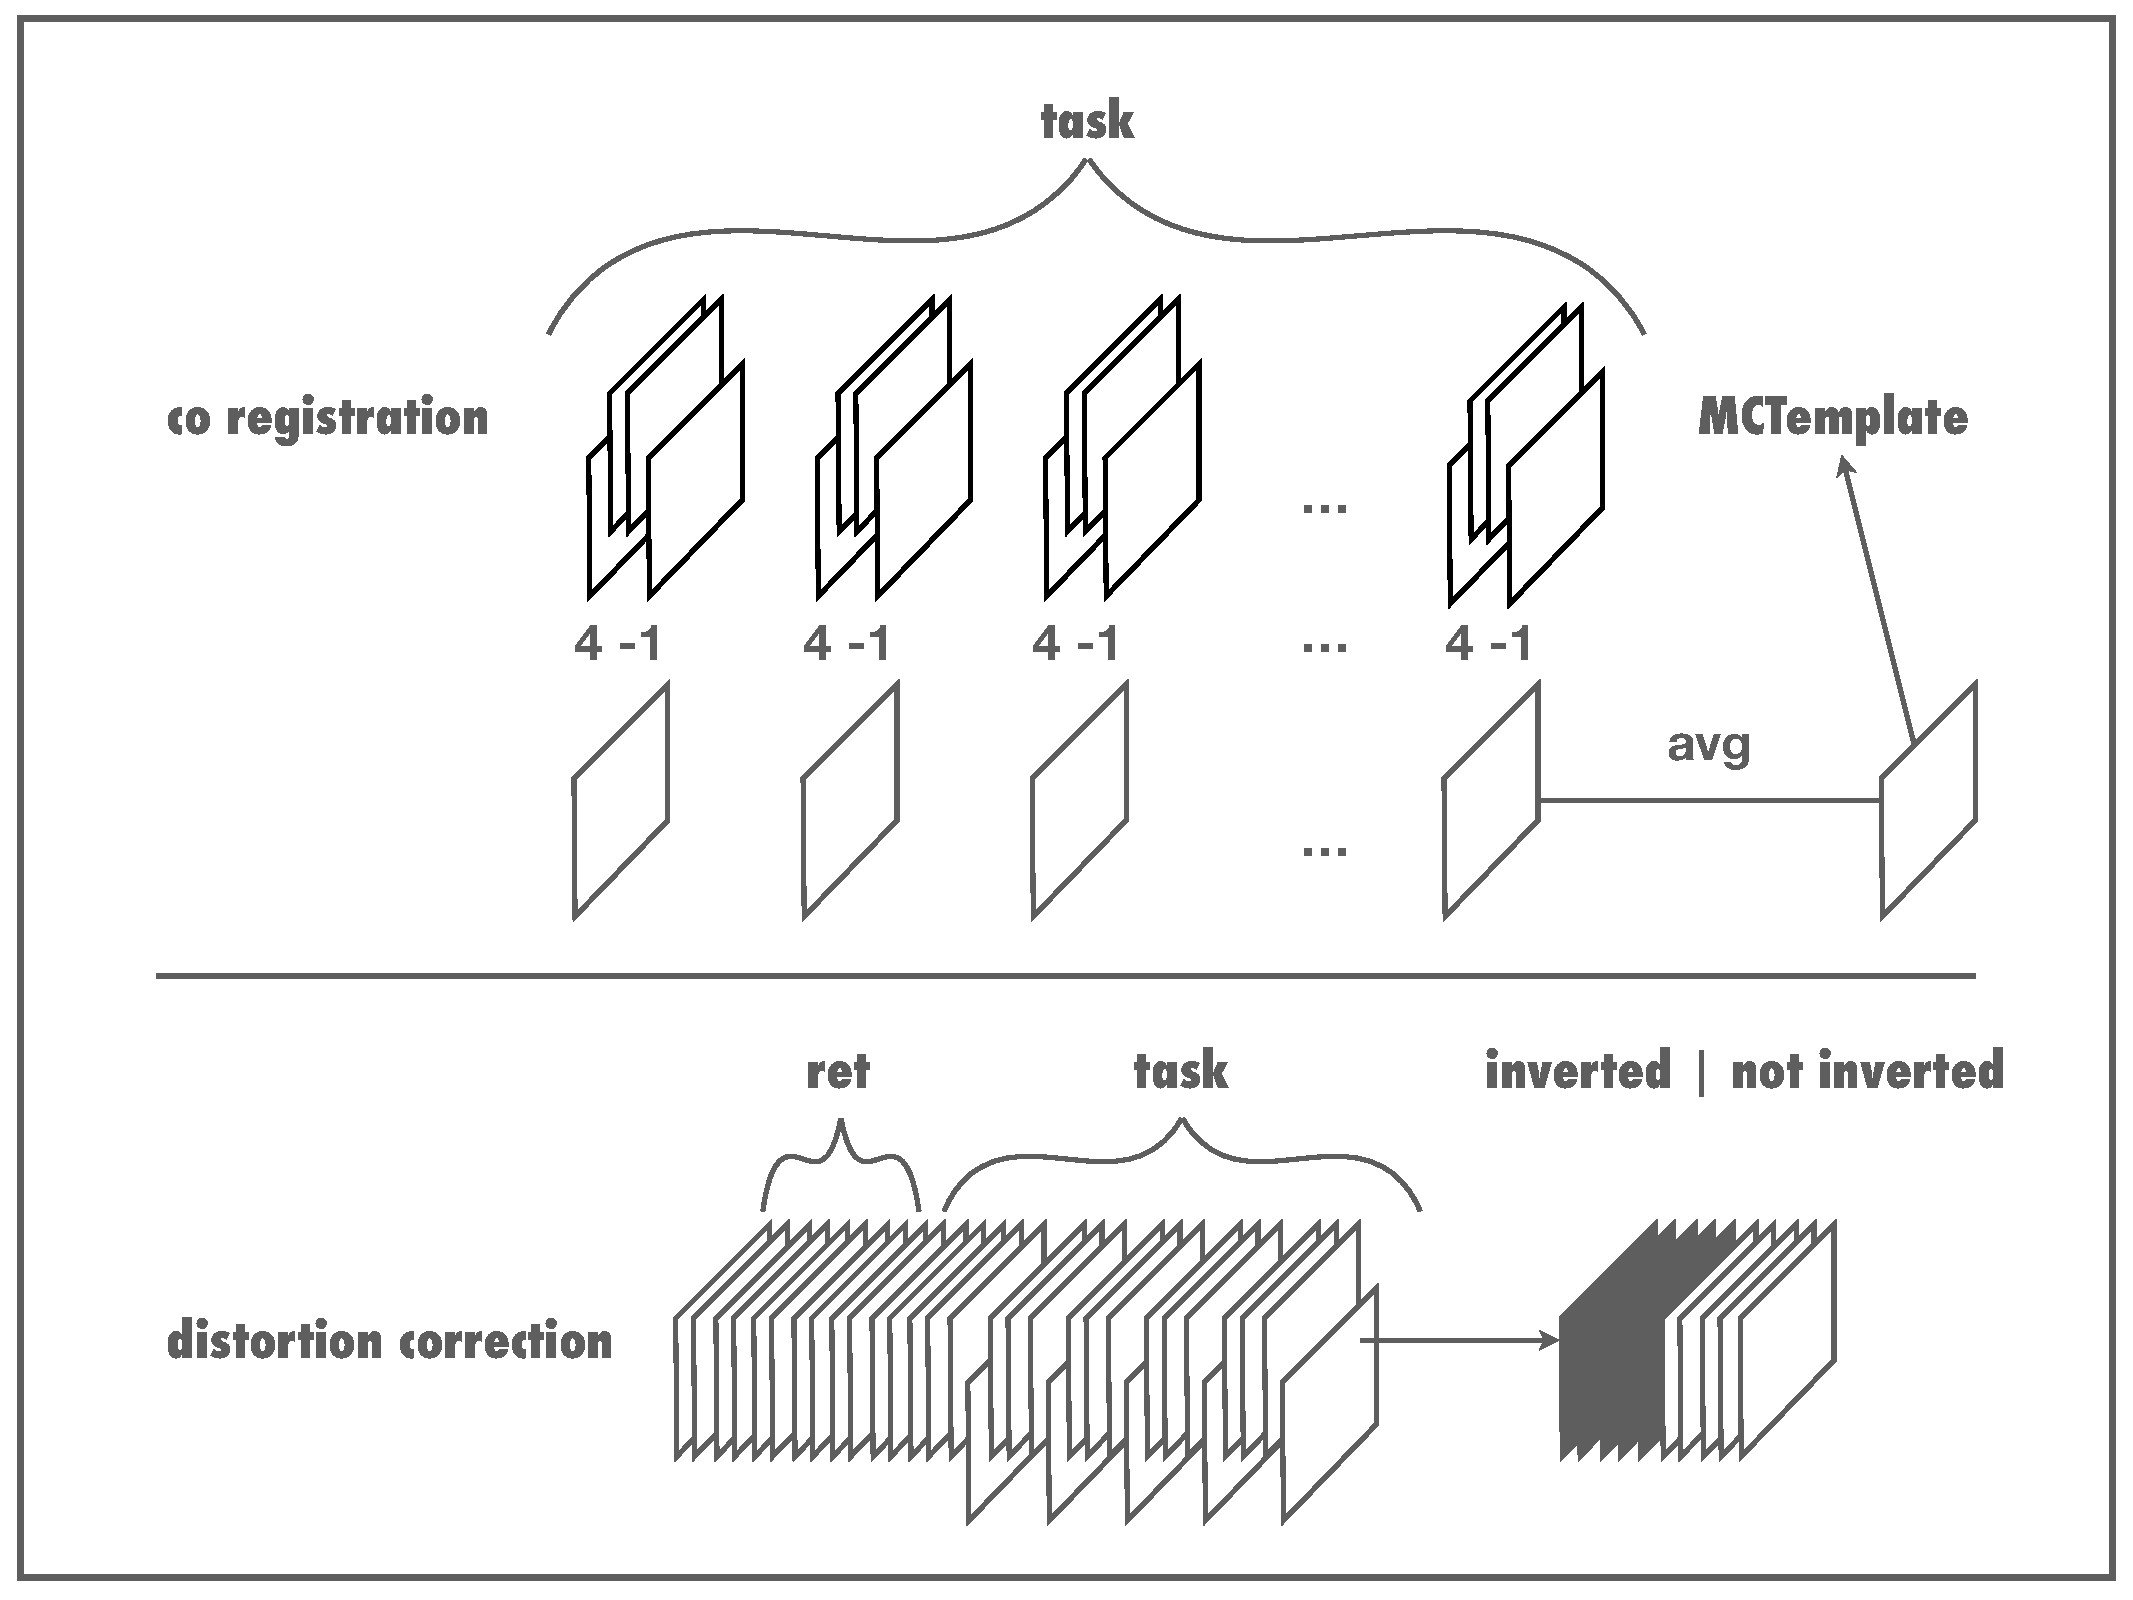
\includegraphics[width=0.8\textwidth]{coregdist}
\caption[Coregistration and distortion correction visual depiction]{Coregistration and distortion correction visual depiction}
\label{fig:coregdist}
\end{center}
\end{figure}

\subsection{fMRI pRF mapping}
Population receptive field mapping. Estimates retinotopic mapping from screen to cortical locations. This is to be done in order to obtain boundaries for visual areas such as V1, V2 and V3. First the fMRI time series will be interpolated (cubic) to match the numeber of frames presented during the stimulation. Afterwards pRF mapping will be analyzed and paramters will be written to volume files (NIfTI) and surface files for use with FreeSurfer.
\begin{table}[h]
%\centering
\begin{tabular}{l | r}
\toprule
maximum memory required & approx time required\\\toprule
64GB (480GB) & $\approx 8h$ \\\bottomrule
\end{tabular}
\end{table}
\FloatBarrier
\noindent Interpolate time series of volumes to match the number of presented frames during stimulation, by resampling the TR to match the "stimulation-frame-rate". Which means the change rate of the stimlus and eventual blank frames. The function below submits the corresponding MATLAB script as a qsub job.\\
The data will furthermore be transformed into percent change relative to the mean. If the new TR (relative to "stimulation-frame-rate") is eqial to the original TR, no interpolation will be applied.\\

\noindent Results can be found in 4\_retinotopy/\\
\begin{lstlisting}[
    language=Shell,
    basicstyle=\ttfamily,
    breaklines=true]
    # interpolate volume time series
    sh do_tseriesinterpolation.sh
\end{lstlisting}
Once the data is in the right space to estimate voxel activity, based on active screen pixels, population receptive field mapping can be performed. Since using high resolution fMRI leads inevitably to "big data" the analysis has to be split up into multiple parts. In the present case an assumed computation time of $\approx 8h$ is reached by splitting up the analysis into 80 parts. Hence there is a linear relationship between processing time and parts the data can be split up to. In the present case all together $480~GB$ of memory are used to perform the analysis in parallel on 80 different cluster nodes with only $6~GB$ each. Afterwards results are combined into a single results file and temporary results are deleted.\\

\noindent Results can be found in 4\_retinotopy/\\
\begin{lstlisting}[
    language=Shell,
    basicstyle=\ttfamily,
    breaklines=true]
    # perform pRF mapping by splitting up the search space of voxels and combining the results.
    sh do_split_analyzePRF.sh
    sh combine_split_PRF_results.sh
\end{lstlisting}
After for each voxel certain parameters like circular coordinates mapping to screen locations, those have to be transformed into volumes, that can be overlayed with anatomical data in order to define masks for regions of interest based on the pRF mapping.\\

\noindent Results can be found in 4\_retinotopy/\\
\begin{lstlisting}[
    language=Shell,
    basicstyle=\ttfamily,
    breaklines=true]
    # transform pRF mapping results into NIfTI volume overlays
    sh make_PRF_overlays.sh
    sh runonqsub.sh 16gb makeOverlays.sh
\end{lstlisting}

\subsection{fMRI layer segmentation}
Gray matter boundaries will be used to compute cortical layer separation. First tksurfer is used to "draw" occipital ROIs based on the retinotopic mapping. Those regions will be transformed into gray matter masks such that an individual masks for V1, V2, V3 for each hemisphere exists. Cortical layer separation yields a probability map for each voxel to lay within a specifcially spaced area between gray matter boundaries. Thus a layer specific ROI specific map is created for each ROI by multiplying the ROI map with each of the layer probability maps. The results are 4D mask volumes separating the layer probabilies in the 4th dimension.
\begin{table}[h]
%\centering
\begin{tabular}{l | r}
\toprule
maximum memory required & approx time required\\\toprule
16GB & $\approx 0.5h+user$ \\\bottomrule
\end{tabular}
\end{table}
\FloatBarrier
FreeSurfer's tksurfer (\href{https://surfer.nmr.mgh.harvard.edu/fswiki/TkSurfer}{\nolinkurl{https://surfer.nmr.mgh.harvard.edu/fswiki/TkSurfer}}) is used to obtained visual ROIs from retinotopic mapping. When running \texttt{\nameref{sh:GUI2ROI}}, an instance of tksurfer is spawned with the correct overlay already set up. In some cases the required 0\_freesurfer/mri/orig.mgz is not present, but instead it's called orig\_nu.mgz. In that case please make sure that 0\_freesurfer/mri/orig.mgz exists by copy-pasting orig\_nu.mgz to orig.mgz This can also be achieved by calling:\\
\begin{lstlisting}[
    language=Shell,
    basicstyle=\ttfamily,
    breaklines=true]
    # cd to /B_scripts folder
    cp ../0_freesurfer/mri/orig_nu.mgz  ../0_freesurfer/mri/orig.mgz
\end{lstlisting}
Afterwards run the commands below again. Once the overlay is displayed correctly, proceed as described in Section~\ref{sec:GUIprf}. Afterwards labels are transformed into masks. Since the selection was done on a surface, the corresponding mask volume is only one voxel thick. Hence voxel have to be expanded to fill the gray matter area.\\

\noindent Results can be found in 5\_laminar/\\
\begin{lstlisting}[
    language=Shell,
    basicstyle=\ttfamily,
    breaklines=true]
    # making masks for V1,2,3 based on retinotopy
    sh GUI2ROIs.sh
    sh labels2masks.sh
    sh expandROIs.sh
\end{lstlisting}
\begin{figure}
\begin{center}
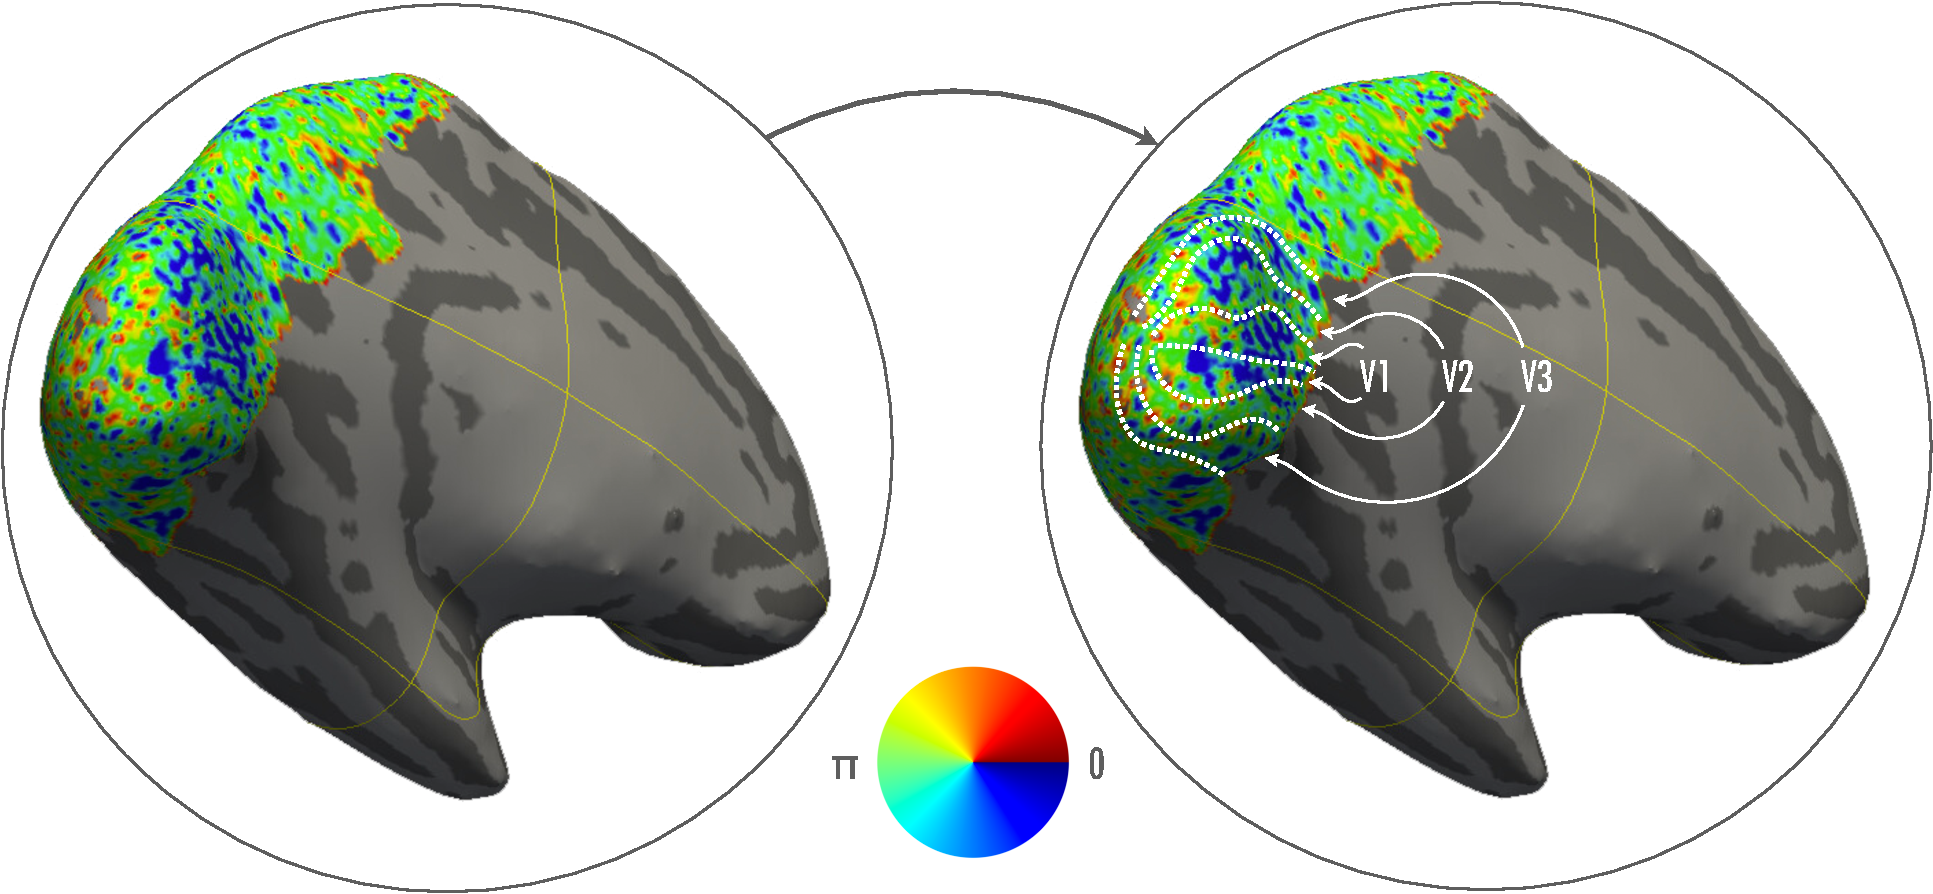
\includegraphics[width=1\textwidth]{ROIselpRF}
\caption[Example for visual ROI definition]{Definition of visual ROIs. Note that along the borders of visual areas a significant shift in color occurs.}
\label{fig:ROIpRF}
\end{center}
\end{figure}
Note that using FreeSurfer's freeview yields better plotting functionality, however \texttt{tksurfer} provides an easier way to select vertices.\\
Once this is done gray matter volumes are split into corical layers. This is implemented in OpenFmriAnalysis (\href{https://github.com/TimVanMourik/OpenFmriAnalysis}{\nolinkurl{https://github.com/TimVanMourik/OpenFmriAnalysis}}). Based on gray and white matter boundaries and the respective curvature, gray matter is segmented into 3 layers. The result is a probability map for each voxel to belong to a certain layer.\\

\noindent Results can be found in 5\_laminar/\\
\begin{lstlisting}[
    language=Shell,
    basicstyle=\ttfamily,
    breaklines=true]
    # performing laminar separation
    sh do_getLayers.sh
    sh do_getLayerWeights.sh
\end{lstlisting}

After the data was computed it is optional to call \texttt{sh \nameref{sh:makeMov}} to create a movie file in C\_miscResults slicing through the volume overlayed with the layer boundaries.
\FloatBarrier

\subsection{fMRI last steps}
The last step is to combine all previously computed results into a single MATLAB file for later staistical analyses using \texttt{\nameref{sh:fMRI}}.\\

\noindent Results can be found in 7\_results/\\
\begin{lstlisting}[
    language=Shell,
    basicstyle=\ttfamily,
    breaklines=true]
    # finalize results
    sh do_finalizeMRIprocessing.sh
\end{lstlisting}


\subsection{EEG pre-processing}
The raw EEG signal will be transformed into virtual channel data by applying a LCMV beamformer. Frequencies of interest ($\alpha$, $\beta$, $\gamma$) are defined that $8~Hz \leq \alpha \leq 12~Hz$; $18~Hz \leq \beta \leq 28~Hz$; $60~Hz \leq \gamma \leq 80~Hz$. Since the covariance matrices of the noise will differ significantly for lower and higher frequencies, the data will be band pass filtered for low and high frequencies separately. This will be achieved by using pass bands of $2-32~Hz$ and $30-100~Hz$ respectively.\\
A FEM forward model will be used as well as a anatomical constraint source model (see Figure~\ref{fig:exampleSourcemodel} for a graphical depiction).\\
\begin{table}[h]
%\centering
\begin{tabular}{l | r}
\toprule
maximum memory required & approx time required\\\toprule
$16~GB$ & $\approx 2h$ \\\bottomrule
\end{tabular}
\end{table}
First data is loaded an segmented into trials. Note that the default trial selection string might vary from experiment to experiment. Target trigger values can be set in \texttt{\nameref{sh:EEGpreproc}}\\
Additionally the data will be band pass filtered at $2-32~Hz$ for $\alpha$ and $\beta$ bands and at $30-100~Hz$ for $\gamma$. Respective changes in the filterband can be made in \texttt{\nameref{sh:EEGpreproc}}\\
If desired, trials should be excluded at this stange as well. To achieve this either use FieldTrip's built in functionality (\texttt{\nameref{sh:EEGpreproc}} bottom) or provide a logical array of whether to include a trial to \texttt{ft\_redefinetrial(cfg, data)}. See \href{http://www.fieldtriptoolbox.org/reference/ft_redefinetrial}{\nolinkurl{http://www.fieldtriptoolbox.org/reference/ft\_redefinetrial}} for more information.\\

\noindent Results can be found in 6\_EEG/\\
\begin{lstlisting}[
    language=Shell,
    basicstyle=\ttfamily,
    breaklines=true]
    # EEG preprocessing: trial selection, BP filter, (trial selection)
    sh do_EEGpreprocessing.sh
\end{lstlisting}
Once the general preprocessing is done, the function \texttt{ft\_timelockanalysis} (\href{http://www.fieldtriptoolbox.org/reference/ft\_timelockanalysis}{\nolinkurl{http://www.fieldtriptoolbox.org/reference/ft\_timelockanalysis}}) is used to estimate the noise covariance matrix based on baseline data for high and low frequencies separately. This is necessary since the noise structure for those different bands varies significantly. The default noise estimation window is $-0.5$ to $-0.1~s$ realtive to stimulus onset.\\

\noindent Results can be found in 6\_EEG/\\
\begin{lstlisting}[
    language=Shell,
    basicstyle=\ttfamily,
    breaklines=true]
    # EEG preprocessing: noise estimation
    sh do_EEGtimelock.sh
\end{lstlisting}
As last step the result from \texttt{fsrecon} (\texttt{\nameref{sh:fsrecon}}) must be prepared to be used as source model. For this purpose Workbench (\href{https://github.com/Washington-University/workbench}{\nolinkurl{https://github.com/Washington-University/workbench}}) is used, wrapped into \texttt{\nameref{sh:prepFS4EEG}}\\

\noindent Results can be found in 6\_EEG/\\
\begin{lstlisting}[
    language=Shell,
    basicstyle=\ttfamily,
    breaklines=true]
    # EEG preprocessing: source model preparation
    sh do_EEGprepareFS.sh
\end{lstlisting}


\subsection{EEG prepare head and source models}
Head and Sourcemodel are prepared using FieldTrip. Per default the pipeline is set up to use finite element models (FEM), but can be changed to boundary element model (BEM) as well. As source model, the result from Workbench is used.
\label{sec:Sourcemodel}
\begin{table}[h]
%\centering
\begin{tabular}{l | r}
\toprule
maximum memory required & approx time required\\\toprule
$32~GB$ & $\approx 6h+user$ \\\bottomrule
\end{tabular}
\end{table}
Loading and segmenting anatomical MRI data is done using ft\_volumesegment (\href{http://www.fieldtriptoolbox.org/reference/ft\_volumesegment}{\nolinkurl{http://www.fieldtriptoolbox.org/reference/ft\_volumesegment}}) and \texttt{ft\_prepare\_mesh} (\href{http://www.fieldtriptoolbox.org/reference/ft\_prepare\_mesh}{\nolinkurl{http://www.fieldtriptoolbox.org/reference/ft\_prepare\_mesh}}). For more details about the settings of this function see Section~\ref{sh:prepHM}.\\

\noindent Results can be found in 6\_EEG/\\
\begin{lstlisting}[
    language=Shell,
    basicstyle=\ttfamily,
    breaklines=true]
    # prepare head model
    sh do_EEGprepareHeadmodel.sh
\end{lstlisting}
Once the headmodel is prepare, sensor locations need to be coregistered. This is achieved by starting an interactive MATLAB session and opening the script \texttt{\nameref{m:elecReg}}. The FieldTrip function \texttt{ft\_electroderealign} is used to interactively coregister sensor locations to anatomical MR data. See \href{http://www.fieldtriptoolbox.org/reference/ft\_electroderealign}{\nolinkurl{http://www.fieldtriptoolbox.org/reference/ft\_electroderealign}} for more information.\\

\noindent Alternatively electrodes can be obtained differently (e.g. using photogrammetry and \texttt{\nameref{sec:janus3D}}). See Section~\nameref{sec:HTphotogr} for more information on that. If using alternative EEG electrode locations, the respective line in \texttt{\nameref{m:elecReg}} must be changed. In case janus3D electrodes are used the step below can also be skipped, if the respective electrode file is already in the correct location.

\begin{lstlisting}[
    language=Shell,
    basicstyle=\ttfamily,
    breaklines=true]
    # coregister electrode locations to anatomical MR using MATLAB
    matlab
\end{lstlisting}
The previously computed data is now prepared to be finally used and the Workbench sourcemodel is loaded.\\

\noindent Results can be found in 6\_EEG/\\
\begin{lstlisting}[
    language=Shell,
    basicstyle=\ttfamily,
    breaklines=true]
    # prepare data and load source model
    sh do_EEGprepareSourcemodel.sh
\end{lstlisting}
\begin{figure}
\begin{center}
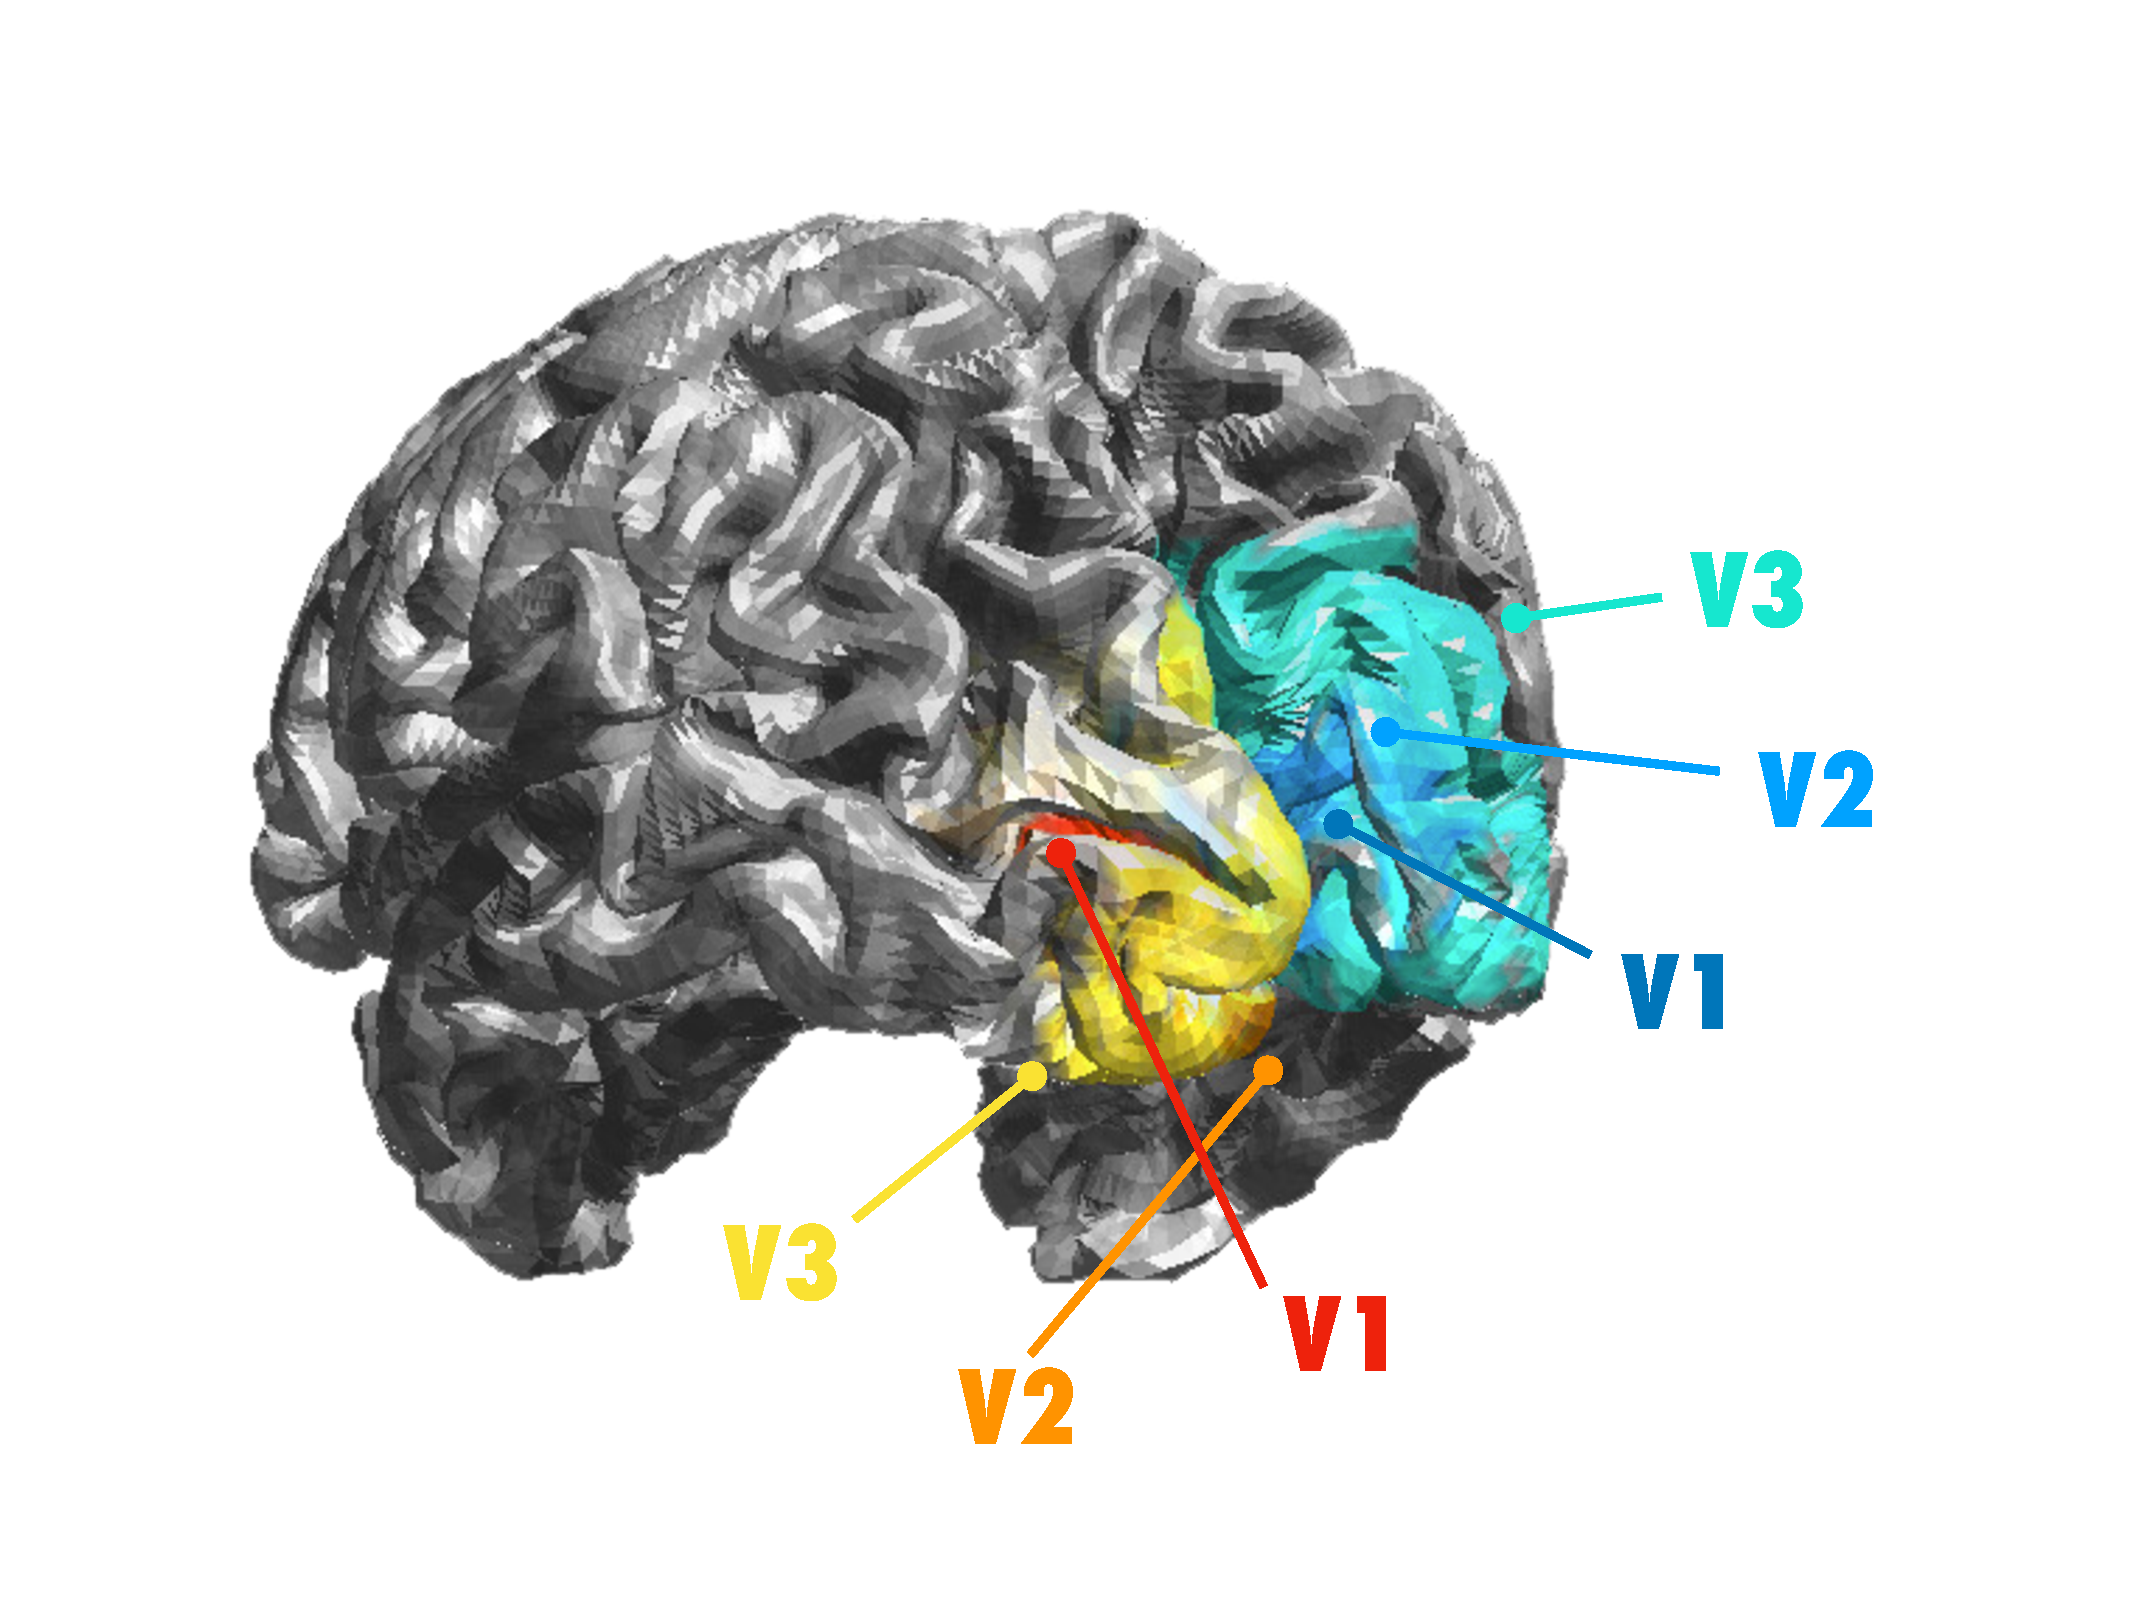
\includegraphics[width=0.8\textwidth]{exampleSourcemodel}
\caption[Example source model]{Example source model including visual ROIs. Note that for demonstrative purposes all possible ROIs are show, however per default only V1 for both hemispheres will be used. This plot was created using \texttt{\nameref{m:visVirtChan}}}
\label{fig:exampleSourcemodel}
\end{center}
\end{figure}
\FloatBarrier
\subsection{EEG compute virtual channels}

\begin{table}[h]
%\centering
\begin{tabular}{l | r}
\toprule
maximum memory required & approx time required\\\toprule
$960~GB$ & $\approx 12h$ \\\bottomrule
\end{tabular}
\end{table}
The first step is to estimate time courses for dipoles at each voxel lcoation. To achieve this LCMV beamformer weights are computed separately for high and low frequencies. To reduce search space and hence computation time, previously computed ROI maps are used. By default left and right V1 are used as two separate ROIs. Volumetric ROIs are translated into cartesian coordinates. Beamformer weights are computed using \texttt{$\lambda=10\%$} for noise regularization employing \texttt{ft\_sourceanalysis} (\href{http://www.fieldtriptoolbox.org/reference/ft\_sourceanalysis}{\nolinkurl{http://www.fieldtriptoolbox.org/reference/ft\_sourceanalysis}}). Trial segmented data is then multiplied with beamformer weights, in order to obtain individual time series for all dipole locations.\\
Note that $480~GB$ of memory are required to estimate the beamformer weights in a parallelized fashion as below.\\

\noindent Results can be found in 6\_EEG/\\
\begin{lstlisting}[
    language=Shell,
    basicstyle=\ttfamily,
    breaklines=true]
    # prepare data and load source model
    sh do_EEGsplitBeamformer.sh
    sh do_EEGsplitVirtualChannel.sh
\end{lstlisting}
Afterwards a time frequency analysis (\href{http://www.fieldtriptoolbox.org/reference/ft\_freqanalysis}{\nolinkurl{http://www.fieldtriptoolbox.org/reference/ft\_freqanalysis}}) is run for all virtual channels. Since this operation is performed on a single trial basis for different filter bands and left and right hemisphere separately, $960~GB$ of memory are required to compute this step as implemented.\\

\noindent Results can be found in 6\_EEG/\\
\begin{lstlisting}[
    language=Shell,
    basicstyle=\ttfamily,
    breaklines=true]
    # prepare data and load source model
    sh do_EEGsplitFreqOnVirtChan.sh
\end{lstlisting}
To relate the data to layer specific fMRI results, a channel selection has to take place, that is optimized for frequency ROIs ($\alpha, \beta, \gamma$). For each of the 3 bands all virtual channels will be searched and the best 100 are selected. Those are defined to have the lowest ($\alpha, \beta$) or highest ($\gamma$) relative power compared to the baseline period ($-0.3$ to $-0.2~s$ relative to simulus onset).\\

\noindent Frequency ROIs are defined as:
\begin{table}[h]
%\centering
\begin{tabular}{c | c | c}
\toprule
$\alpha$ & $\beta$ & $\gamma$\\\toprule
$8-12~Hz$ & $22-28~Hz$ & $50-70~Hz$ \\\bottomrule
\end{tabular}
\end{table}\\
Furthermore, the function produces figures saved in C\_miscResults similar to what is shown in Figure~\ref{fig:exampleGamma}.\\

\noindent Results can be found in 7\_results/\\
\begin{lstlisting}[
    language=Shell,
    basicstyle=\ttfamily,
    breaklines=true]
    # prepare data and load source model
    sh do_EEGfreqChanSelect.sh
\end{lstlisting}
\begin{figure}
\begin{center}
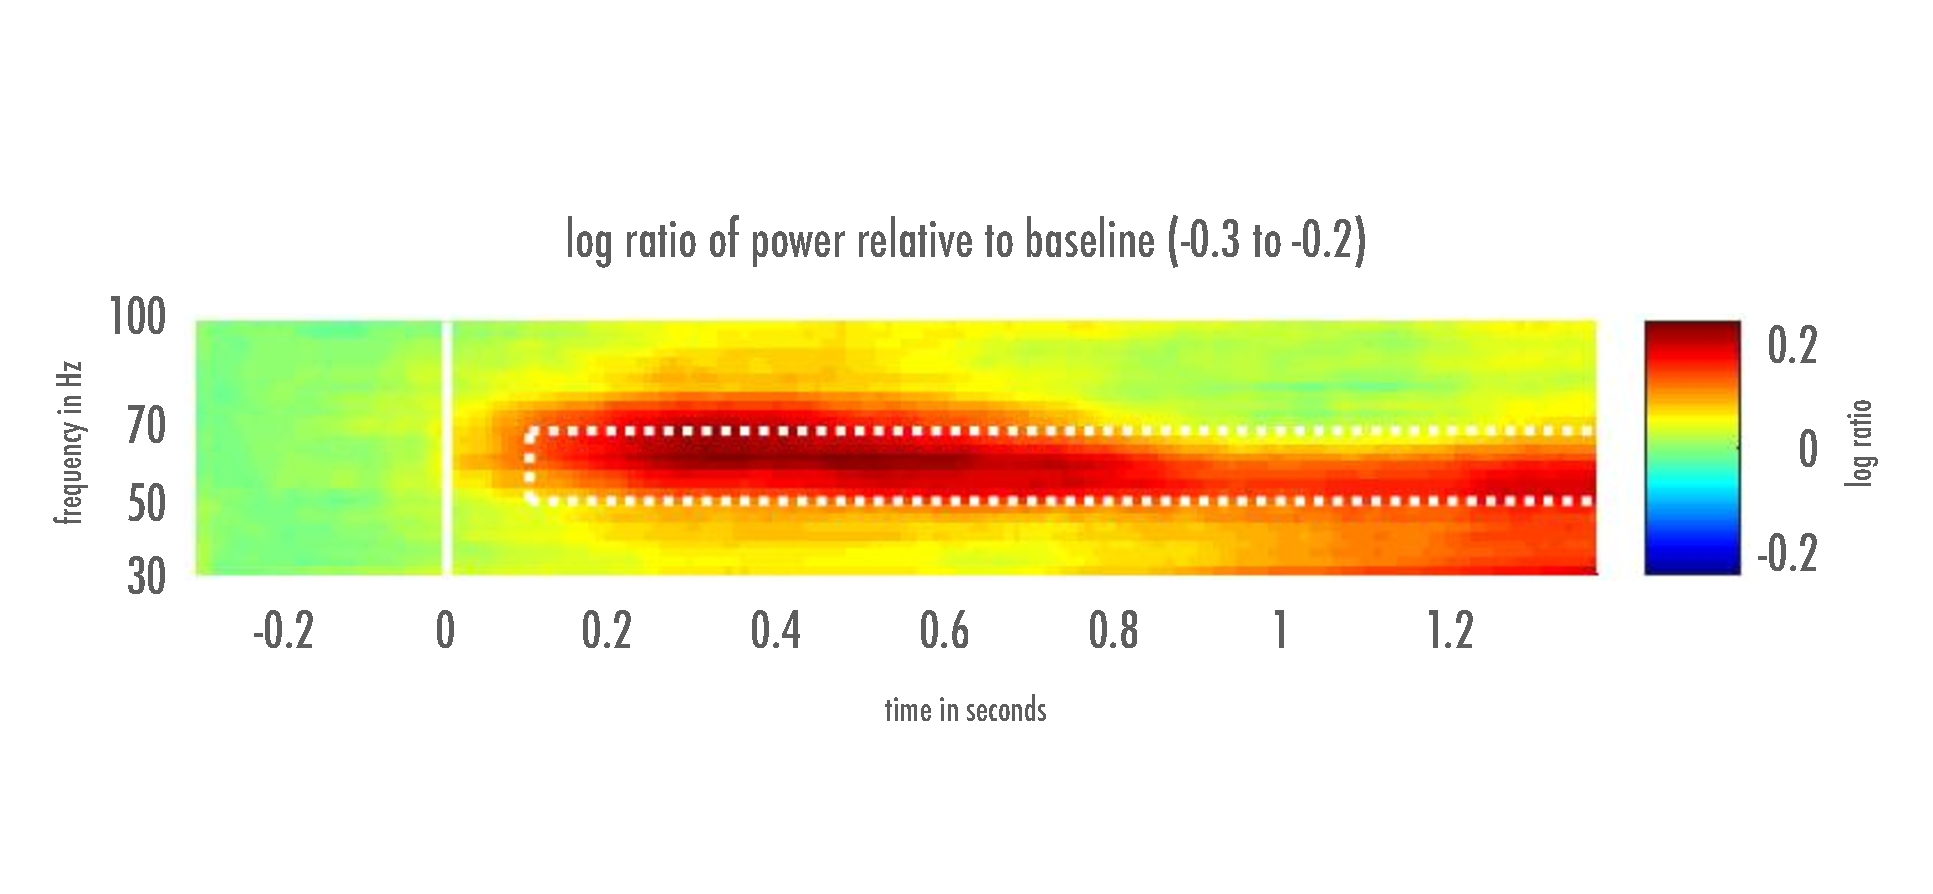
\includegraphics[width=1\textwidth]{exampleGamma}
\caption[Example for $\gamma$ response in virtual channel]{Example for $\gamma$ response in virtual channel}
\label{fig:exampleGamma}
\end{center}
\end{figure}

\subsubsection{EEG-fMRI combined analysis}
Combined analysis is not yet part of this documentation. MATLAB scripts starting with \texttt{stats\_} or \texttt{fun\_} belong to this part. Those were provided by Rene Scheeringa (DCCN, 2018) and adapted to work integratively with the rest of the pipeline. However, since the integration is not fully finished yet, the respective parts were omitted from the documentation for now.

\subsection{Ultra lazy}
It is quite nocticable, that large chunks can be grouped together. For this purpose some meta-scripts are included as well, that are not documented, because it is not recommended going that way. It's better to call the scripts squentially in order to spot probable errors as early in the pipeline as possible. However, once everything is set up, an entire single subject (after preparation) can be run using the following scripts:
\begin{lstlisting}[
    language=Shell,
    basicstyle=\ttfamily,
    breaklines=true]
    # prepare fMRI data
    sh runonqsub.sh 32gb do_preparefunctionals.sh

    # prepare FreeSurfer
    sh runonqsub.sh 16gb do_fsrecon.sh
    sh do_EEGprepareFS.sh

    # process EEG (& to not wait for completion)
    sh EEG_preprocessing.sh &

    # MRI preprocessing part 1
    sh MRI_preprocessing_part1of2.sh

    # check if MCTemplateThrCont.nii looks good using e.g. fsleyes

    # MRI preprocessing part 2
    sh MRI_preprocessing_part2of2.sh

    # define V1,2,3
    sh GUI2ROIs.sh

    # MRI layer segmentation
    sh MRI_postprocessROIs.sh

    # finilize processing
    sh do_finalizeMRIprocessing.sh
\end{lstlisting}
\FloatBarrier

\section{Scripts explained (support for runonqsub.sh: Q)}
\label{sec:scriptsExplained}
\subsection{cleanscriptsfolder.sh}
\label{sh:clean}
Since qsub puts a output + error log into /B\_ scripts \texttt{\nameref{sh:clean}} can be used to move all qsub outputs to /B\_scripts/qsuboutput\\

\subsection{combine\_split\_PRF\_results.m}
\label{m:combsplt}
Combines split results from \texttt{\nameref{sh:splitanalyzePRF}} (Section~\ref{sh:splitanalyzePRF}) into a single MATLAB file. Note that given the respective numerical naming of all parts (x\_of\_X) parts will be concatenated along values of x. After this operation split parts will be deleted.\\

\subsection{combine\_split\_PRF\_results.sh}
\label{sh:combsplt}
Wrapper function for running \texttt{\nameref{m:combsplt}} via qsub. Combines split results from \texttt{\nameref{sh:splitanalyzePRF}} (see Section~\ref{sh:splitanalyzePRF}). Note that the exact amount of parts that the data was split into must be defined here (default: 80).\\

\subsection{do\_analyzePRF.m}
\label{m:analyzePRF}
Computes pRF mapping implemeting "analyzePRF" from the analyzePRF toolbox. It can be decided whether to average across blocks or if the estimates shall be done for each block separately and averaging the results. Note, that running the analysis on separate blocks slows down computation time, but to my experience yields slightly better results.\\

\noindent Under the hood:
\begin{itemize}
\item estimates pRFs
\item computes pRF mapping for part x of X by splitting the list of indices and selecting the corresponding set
\item set avgdata=1 to average data before the analysis (otherwise it will be averaged afterwards)
\item result: structure containing pRF parameters of part x of X
\end{itemize}

\subsection{do\_analyzePRF.sh}
\label{sh:analyzePRF}
Wrapper function for running \texttt{\nameref{m:analyzePRF}} via qsub. Spawns a qsub job using 6GB of memory (default) and runs a specific part of a set of parts. The first input argument is the part that is to be computed and the second input argument is the sum of all parts.
\begin{lstlisting}[
    language=Shell,
    basicstyle=\ttfamily,
    breaklines=true]
    # example split search space into 5 parts an run the first
    sh do_analyzePRF.sh 1 5
\end{lstlisting}
\begin{lstlisting}[
    language=Shell,
    basicstyle=\ttfamily,
    breaklines=true]
    # example not splitting up search space
    sh do_analyzePRF.sh 1 1
\end{lstlisting}

\subsection{do\_applysimpledistcorr.sh (Q)}
\label{sh:applydistcorr}
Applies distortion correction to all functional data.\\

\noindent Under the hood:
\begin{itemize}
\item distortion correction is applied to the full set of functionals using the \texttt{OUTPUT} of topup (\texttt{topup [$\ldots$] --out=OUTPUT}) as well as acquisition\_parameters.txt (Using \texttt{--method=jac})
\item all results are stored in /2\_distcorrection
\item all results have the prefix "corrected\_"
\end{itemize}

\subsection{do\_coregistration.m}
\label{m:coreg}
The script doing the actual co-registration. Uses wrapper functions from OpenFmriAnalysis to evoke FreeSurfers \texttt{bbregister} and computes a recursive boundary based registration.\\

\noindent The results are several files storing the boundaries as a point cloud, and the respective transformation in different formats.

\noindent Under the hood:
\begin{itemize}
\item calls \texttt{bbregister}
\item results are stored in /3\_coregistration
\item yields boundaries.mat, matrix.mat, bbregister.dat, transmat.txt, transmatinv.txt
\end{itemize}

\subsection{do\_coregistration.sh}
\label{sh:coreg}
Wrapper function for running \texttt{\nameref{m:coreg}}, that in turn will be using FreeSurfer (\texttt{bbregister}) and OpenFmriAnalysis to perform a linear and non-linear boundary registration.  Movie files of the respective co-registration are stored in /C\_miscResults.\\

\subsection{do\_correctavgdiff.sh (Q)}
\label{sh:corravg}
Due to the subtraction of the 1st from the 3rd volume the area outside the brain has the highest value. In order to correct this the lowest value will be shifted to zero the a certain part of the higher values are cut (e.g. 0.975).\\

\noindent The result should be checked using\\
\texttt{fsleyes ../3\_coregistration/Inplane/MCTemplateThr*.nii.gz} to ensure that the area outside the brain is nulled. Note that it can happen that some areas within the brain are nulled as well. If they are not too wide spread they do not affect later co-registration.\\

\subsection{do\_distcorr.sh (Q)}
\label{sh:distcorr}
Uses the averge volume of the inverted set of images in /niftis/inverted as reference for \textit{inverted}\\

\noindent Uses as many volumes \textit{n} as there were in /niftis/inverted. Respective volumes are selected starting from the last going in \textit{3 x n} steps backward. Hence the resulting average of this set was computed over the 3rd volume of each of \textit{n} last sets in the normal images. Simplified (all 1 are selected):\\

\noindent for n=5\\

\noindent 0,0,0,0,...,0,0,0,0,0,0,0,1,0,0,1,0,0,1,0,0,1,0,0,1\\

\noindent Both (normalavg and invertedavg) will be used to esimate the distortion correction.\\

\noindent Under the hood:
\begin{itemize}
\item reference volumes (normal + inverted) are selected in order to do the field distortion estimate (selection: see above).
\item selected reference volumes are merged into a single file (/2\_distcorrection/all\_b0.nii.gz)
\item topup is called using the merged (normal + inverted) .nii and performs field mapping accoriding to the specifications in /A\_helperfiles/b02b0.cnf using the acquisition parameters specified in acquisition\_parameters.txt
\item all results are stored in /2\_distcorrection
\end{itemize}

\subsection{do\_EEGbeamformer.m}
\label{m:beamf}
\begin{lstlisting}[
    language=Matlab,
    basicstyle=\small,
    breaklines=true]
    Selprefix = 'TL';
    Addprefix='Beamf_centV1_';
\end{lstlisting}
Performing LCMV beamforming on the data. Since the grid size will be scaled to match the functional (high-res) data, scanning the full space would require too much computation time. Hence a ROI mask is used, that is in the present case the white matter voxels in V1, as obtained from retinotopy scans. Noise regularization was set to $\lambda=10\%$\\

\subsection{do\_EEGbeamformer.sh}
\label{sh:beamf}
Wrapper function for running \texttt{\nameref{m:beamf}} via qsub.\\

\subsection{do\_EEGelectrodeRegistration.m}
\label{m:elecReg}
This function cannot be run using Qsub or a headless MATLAB instance, since it requires user interaction via a graphical user interface. The script will load the respective data, save and exit (after the user is done). Since this script is just a wrapper function for \texttt{ft\_electroderealign} I will refer to the corresponding FieldTrip documentation: \href{http://www.fieldtriptoolbox.org/reference/ft\_electroderealign}{\nolinkurl{http://www.fieldtriptoolbox.org/reference/ft\_electroderealign}}\\

\noindent However there is the option to specify a custom path to stored EEG electrodes. By default this is thought to be the result of \texttt{janus3D}. For more information on that see Section~\nameref{sec:janus3D}.

\subsection{do\_EEGfreqChanSelect.m}
\label{m:selchan}
\begin{lstlisting}[
    language=Matlab,
    basicstyle=\small,
    breaklines=true]
    Selprefix='TF';
    % Addprefix=''; does not exist
\end{lstlisting}
Selects virtual channels of interest. Since utilizing high resolution functional data is leading inevitably to an explosion in file size, only important data will remain after calling this function.\\

\noindent First of all it is specified which are the frequency bands of interest in order to make a choise for a respective channel to maximize or minimize within the defined range. Default settings are:
\begin{lstlisting}[
    language=Matlab,
    basicstyle=\small,
    breaklines=true]
    ROIalpha = [8,12]; % Hz
    ROIbeta  = [22.5,27.5]; % Hz
    ROIgamma = [50,70]; % Hz

    timeWinMax = [0.1 1.39]; % in seconds
\end{lstlisting}

\texttt{timeWinMax} thereby is the time of interest for which to optimize channel selection. Shortly speeking an area within the time frequncy matrix that is enclosed by \texttt{ROI$<$freq$>$} and \texttt{timeWinMax} will be averaged. The 100 maximum (for $\gamma$) and minimum (for $\alpha$ and $\beta$) channels will be selected. It is important to note, that the data will be $\log$ transformed and expressed as relative change to \texttt{BLwin} which is the respective time window of reference relative to stimulus onset.\\

\noindent The final MATLAB structure loos like this:

\begin{figure}[h]
\caption{Result of EEG analysis as a MATLAB structure}
\vspace{10pt}
{\scriptsize
\begin{forest}
  for tree={
    font=\ttfamily,
    grow'=0,
    child anchor=west,
    text height=0.01cm,
    parent anchor=south,
    anchor=west,
    calign=first,
    edge path={
      \noexpand\path [draw, \forestoption{edge}]
      (!u.south west) +(12pt,0pt) |- node[fill,inner sep=1.25pt] {} (.child anchor)\forestoption{edge label};
    },
    before typesetting nodes={
      if n=1
        {insert before={[,phantom]}}
        {}
    },
    fit=band,
    before computing xy={l=20pt},
  }
  [VirtChanData
    [ROI (hemisphere and visual ROI)
    ]
    [pos (voxel coordinates)
    ]
    [freqROI (frequencies of interest)
    ]
    [freqROIfreq (frequencies of freqROI)
    ]
    [filterBand (marginal frequencies of band pass filter)
    ]
    [baselineWin (marginal samples of baseline window)
    ]
    [tROI (time of interest)
    ]
    [ft\_freqanalysis (fieldtrip result structure)
    ]
    [results
      [trial (descending ranked channels $N_{channel} \times N_{freqs} \times N_{timebins} \times N_{blocks}$
      ]
      [dimord (order of above)
      ]
      [label (EEG channel labels)
      ]
      [sortAll (sorting indices)
      ]
      [sortord (sorting order)
      ]
      [beamformerWeights (filter weights)
      ]
    ]
  ]
\end{forest}
}
\label{tree:resEEG}
\end{figure}

\subsection{do\_EEGfreqChanSelect.sh}
\label{sh:selchan}
Wrapper function for running \texttt{\nameref{m:selchan}} via qsub.\\

\subsection{do\_EEGfreqOnVirtChan.m}
\label{m:freqVirt}
\begin{lstlisting}[
    language=Matlab,
    basicstyle=\small,
    breaklines=true]
    Selprefix='VirtCh';
    Addprefix='TF_';
\end{lstlisting}
Computes time-frequency analysis for virtual channel data using \texttt{ft\_freqanalysis}. For more information see \href{http://www.fieldtriptoolbox.org/reference/ft\_freqanalysis}{\nolinkurl{http://www.fieldtriptoolbox.org/reference/ft\_freqanalysis}}.\\
\noindent Per default the frequency of interes (FOI) is set to band pass filter width.The resolution is defined by $\frac{1}{slidW}$ where slidW is the respective size of the sliding window used. Default values are 0.4 for high and 0.8 for low filter bands.\\

\noindent All default settings:
\begin{lstlisting}[
    language=Matlab,
    basicstyle=\small,
    breaklines=true]
    cfg.output       = 'pow'; % power of frequency spectrum
    cfg.channel      = 'all';
    cfg.method       = 'mtmconvol'; % multi-taper-method convolution
    cfg.taper        = 'dpss'; % discrete prolate spheroidal sequences
    cfg.foi          = foi; % frequencies of interest
    cfg.pad          = 3.2; % padding at beginning and end of trial
    cfg.tapsmofrq    = 10; % frequency smoothing
    cfg.t_ftimwin    = ones(length(cfg.foi),1).*slidW(counter); % slidW
    cfg.toi          = -1:0.01:2; % time window of interest
    cfg.keeptrials   = 'yes';
\end{lstlisting}

\subsection{do\_EEGfreqOnVirtChan.sh}
\label{sh:freqVirt}
Wrapper function for running \texttt{\nameref{m:freqVirt}} via qsub.\\

\subsection{do\_EEGprepareFS.sh}
\label{sh:prepFS4EEG}
This script was provided by Simon Hom\"olle (DCCN, 2018). Uses Workbench (\href{https://github.com/Washington-University/workbench}{\nolinkurl{https://github.com/Washington-University/workbench}}) to prepare FreeSurfer results for use with the EEG pipeline.\\

\subsection{do\_EEGprepareHeadmodel.m}
\label{m:prepHM}
Creates volume conduction model either as finite-element model (FEM) or boundary element model (BEM). Per default all scripts are set up to use a FEM model. The respective MRI file to use will be 0\_freesurfer/mri/orig\_nu.mgz. If desired the variable \texttt{convertCoordSys} can be set to \texttt{convertCoordSys = 1;} to convert the coordinate system to ctf (otherwise will be ras).\\

Model specific parameters are:
\begin{lstlisting}[
    language=Matlab,
    basicstyle=\small,
    breaklines=true]
    case 'FEM'
        % segmentation parameters
        cfg.output    = {'gray','white','csf','skull','scalp'};
        cfg.scalpsmooth = 10;

        % mesh parameters
        cfg.method = 'hexahedral';
        cfg.shift  = 0.3; % <0.5, is needed so elements are still convex

        % headmodel parameters
        cfg.method = 'simbio';
        cfg.conductivity = [0.33 0.14 1.79 0.01 0.43];

    case 'BEM'
        % segmentation parameters
        cfg.output    = {'brain','skull','scalp'};
        cfg.scalpsmooth = 10;

        % mesh parameters
        cfg.tissue={'brain','skull','scalp'};
        cfg.method = 'projectmesh';
        cfg.numvertices = [1000 2000 3000];

        % headmodel parameters
        cfg.method = 'openmeeg';
        cfg.conductivity = [0.33 0.01 0.43];
\end{lstlisting}

Underlying FieldTrip functions are:
\begin{itemize}
\item ft\_volumesegment (segments anatomical data into distinct structures (e.g. skull))
\item ft\_prepare\_mesh (sets up 3D mesh for head model preparation)
\item ft\_prepare\_headmodel (creates the conductivity model)
\end{itemize}

\subsection{do\_EEGprepareHeadmodel.sh}
\label{sh:prepHM}
Wrapper function for running \texttt{\nameref{m:prepHM}} via qsub. Changing the variable \texttt{Model} will cause the function to produce a different forward model. Possible options are \texttt{Model=FEM} and \texttt{Model=BEM}.\\

\subsection{do\_EEGprepareSourcemodel.m}
\label{m:prepSM}
Sets up sourcemodel (dipole model) for source analysis using the result of \texttt{\nameref{sh:prepFS4EEG}}\\
\noindent It utilizes FieldTrip's \texttt{ft\_prepare\_vol\_sens} to ensure that headmodel and sensors are set up correctly and prepares the source model by reading the Workbench result as a headshape (\texttt{ft\_read\_headshape}).\\

\noindent Note, that if no sensor file was found, but instead a janus3D result, it will be converted into a sensor file and used. The function will error if neither a sens file, nor a electrode file was provided. See \nameref{m:elecReg} for how to create a sensor file and \nameref{sec:janus3D} for more information on this.

\subsection{do\_EEGprepareSourcemodel.sh}
\label{sh:prepSM}
Wrapper function for running \texttt{\nameref{m:prepSM}} via qsub. Changing the variable \texttt{Model} will cause the function to use a different forward model. Possible options are \texttt{Model=FEM} and \texttt{Model=BEM} (must be in accordance with \texttt{\nameref{sh:prepHM}}).\\

\subsection{do\_EEGpreprocessing.m}
\label{m:EEGpreproc}
\begin{lstlisting}[
    language=Matlab,
    basicstyle=\small,
    breaklines=true]
    % for trial and channel selection
    % Selprefix = ''; does not exist
    Addprefix = 'TCsel_';

    % band pass filtering
    Selprefix = 'TCsel';
    Addprefix=['BP' num2str(filterPassBand(1)) '_' num2str(filterPassBand(2)) '_']; % result is e.g. BP2_32_
\end{lstlisting}
Does a basic preprocessing to the data. First trigger values will be extracted and trials are defined according to the specifications in the script. Further only EEG channels are selected. The Data is downsampled to $1024~Hz$. This in-between step is stored. Afterwards the data is further split into different sets of band pass filtered data. Note, that the noise structure will be different for high and low frequencies and thus this step is highly recommendable. Per default two band pass filters are chosen ($2-32~Hz$ and $30-100~Hz$). The baseline period will be from $-0.5~s$ until $-0.1~s$ relative to the stimulus onset. For the high frequency case a dft filter to filter line noise is applied. Using the default version of this function will store the computed data using the respective filter settings as a prefix. However if desired trials can / should be excluded in this step as well.\\

\noindent Under the hood (uses the following fieldtrip functions):
\begin{itemize}
\item ft\_definetrial (sets up trial definition according to predefined trigger values in the data)
\item ft\_preprocessing (selects EEG channel)
\item ft\_redefinetrial (defines channel and creates trials)
\item ft\_resampledata (downsampling)
\item ft\_preprocessing (frequency filters)
\item $[$ft\_rejectvisual (trial rejection)$]$ see also Section~\ref{sec:eye}
\end{itemize}

\subsection{do\_EEGpreprocessing.sh}
\label{sh:EEGpreproc}
Wrapper function for running \texttt{\nameref{m:EEGpreproc}} via qsub.\\

\subsection{do\_EEGsplitBeamformer.sh}
\label{sh:splitbeamf}
Wrapper function for running \texttt{\nameref{sh:beamf}} in multiple instances. The function calls a predefined number of instances of \texttt{\nameref{sh:beamf}} to run on the cluster, submitted using qsub. Per default 8~jobs requesting 62~GB of memory each, will be spawned. This procedure speeds up the processing significantly and would be otherwise impractical.\\

\subsection{do\_EEGsplitFreqOnVirtChan.sh}
\label{sh:splitfreqVirt}
Wrapper function to call \texttt{\nameref{sh:freqVirt}} The function calls a predefined number of instances of \texttt{\nameref{sh:freqVirt}} to run on the cluster, submitted using qsub. Per default 16~jobs requesting 60~GB of memory each, will be spawned. This procedure speeds up the processing significantly and would be otherwise impractical.\\

\subsection{do\_EEGsplitVirtualChannel.sh}
\label{sh:splitvirtch}
Wrapper function for running \texttt{\nameref{sh:virtch}} in multiple instances. The function calls a predefined number of instances of \texttt{\nameref{sh:virtch}} to run on the cluster, submitted using qsub. Per default 8~jobs requesting 30~GB of memory each, will be spawned. This procedure speeds up the processing significantly and would be otherwise impractical.\\

\subsection{do\_EEGtimelock.m}
\label{m:timelock}
\begin{lstlisting}[
    language=Matlab,
    basicstyle=\small,
    breaklines=true]
    sel_ = {'BP30_100','BP2_32'}; % used in a for loop
    Selprefix = sel_{n}; % inside for loop
    Addprefix = 'TL_';
\end{lstlisting}
Average (re-) referencing, timelock analysis and noise covariance estimation for the data. Estimates noise between $-0.5~s$ until $-0.1~s$ relative to the stimulus onset. Basically a wrapper function to call \texttt{ft\_timelockanalysis} using \texttt{cfg.keeptrials = 'yes'}. See \href{http://www.fieldtriptoolbox.org/reference/ft\_timelockanalysis}{\nolinkurl{http://www.fieldtriptoolbox.org/reference/ft\_timelockanalysis}} for more information.\\

\noindent Subsequent processing steps include average referencing and noise covariance estimation based on the variable \textff{noiseEstWin=[-0.5 -0.1];}\\

\subsection{do\_EEGtimelock.sh}
\label{sh:timelock}
Wrapper function for running \texttt{\nameref{m:timelock}} via qsub.\\

\subsection{do\_EEGvirtualChannel.m}
\label{m:virtch}
\begin{lstlisting}[
    language=Matlab,
    basicstyle=\small,
    breaklines=true]
    Selprefix='Beamf_centV1';
    Addprefix='VirtCh_';
\end{lstlisting}
Computes virtual channel time series, by mutliplying the data with the previously computed spatial filters.\\

\noindent Under the hood:
\begin{lstlisting}[
    language=Matlab,
    basicstyle=\small,
    breaklines=true]
    virtual_channels = mean(dataSrc.avg.mom{nonEmptyFilterInd},2)'*currentFilter*squeeze(data.trial{trial}(:,:));
\end{lstlisting}

The data is multiplied with the respective filter, taking the average dipole moment into account.\\

\subsection{do\_EEGvirtualChannel.sh}
\label{sh:virtch}
Wrapper function for running \texttt{\nameref{m:virtch}} via qsub.\\

\subsection{do\_finalizeMRIprocessing.m}
\label{m:fMRI}
Combines all relevant results of the fMRI analysis into a single MATLAB file of the following structure:\\

\begin{figure}[h]
\caption{Result of fMRI analysis as a MATLAB structure}
\vspace{10pt}
{\scriptsize
\begin{forest}
  for tree={
    font=\ttfamily,
    grow'=0,
    child anchor=west,
    text height=0.01cm,
    parent anchor=south,
    anchor=west,
    calign=first,
    edge path={
      \noexpand\path [draw, \forestoption{edge}]
      (!u.south west) +(12pt,0pt) |- node[fill,inner sep=1.25pt] {} (.child anchor)\forestoption{edge label};
    },
    before typesetting nodes={
      if n=1
        {insert before={[,phantom]}}
        {}
    },
    fit=band,
    before computing xy={l=20pt},
  }
  [data
[data (fMRI data $N_{voxel} \times N_{volumes} \times N_{blocks}$)
]
[maskgray (gray matter mask $N_{voxel} \times 1$)
]
[maskwhite (white matter mask $N_{voxel} \times 1$)
]
[maskecc (eccentricity mask $N_{voxel} \times 1$)
]
[transmats (realignment as matrices $4 \times 4$ for all $N_{volumes}$ and $N_{blocks}$)
]
[transvecs (realignment as vectors $1 \times 6$ for all $N_{volumes}$ and $N_{blocks}$)
]
[layerROIs
  [lh
    [V1 (layer weights $N_{voxel} \times N_{layer}$)]
    [V2 (layer weights $N_{voxel} \times N_{layer}$)]
    [V3 (layer weights $N_{voxel} \times N_{layer}$)]
  ]
  [rh
    [V1 (layer weights $N_{voxel} \times N_{layer}$)]
    [V2 (layer weights $N_{voxel} \times N_{layer}$)]
    [V3 (layer weights $N_{voxel} \times N_{layer}$)]
  ]
]
[CSFwhite (weights for CSF(1) and white matter(2) $N_{voxel} \times 2$)
]
]
\end{forest}
}
\label{tree:resMRI}
\end{figure}

\subsection{do\_finalizeMRIprocessing.sh}
\label{sh:fMRI}
Wrapper function for running \texttt{\nameref{m:fMRI}} via qsub.\\

\subsection{do\_fsrecon.sh (Q)}
\label{sh:fsrecon}
Performs segmentation using Freesurfer.\\

\noindent If running on OSX the script assumes:
\begin{lstlisting}[
    language=Shell,
    basicstyle=\ttfamily,
    breaklines=true]
    # FreeSurfer Home Mac
    FREESURFER_HOME=/Applications/freesurfer
\end{lstlisting}

\noindent If running on linux the script assumes:\\
\begin{lstlisting}[
    language=Shell,
    basicstyle=\ttfamily,
    breaklines=true]
    # FreeSurfer Home Linux
    FREESURFER_HOME=/opt/freesurfer/version
\end{lstlisting}

\noindent The target image that is used for the segmentation must be located in /niftis/t1\\

\noindent Under the hood:
\begin{lstlisting}[
    language=Shell,
    basicstyle=\ttfamily,
    breaklines=true]
    recon-all -i rawData/niftis/t1/* -subjid  0_freesurfer -all OutputVolume.nii.gz
\end{lstlisting}
, all results are stored in /0\_freesurfer\\

\subsection{do\_getLayers.m}
\label{m:getLyr}
Utilizes the toolbox OpenFmriAnalysis (\href{https://github.com/TimVanMourik/OpenFmriAnalysis}{\nolinkurl{https://github.com/TimVanMourik/OpenFmriAnalysis}}) to segment \texttt{numLayers} anatomical layers between the gray and white matter boundaries of the volume \texttt{regvol}.\\

\noindent Under the hood:
\begin{lstlisting}[
    language=Matlab,
    basicstyle=\small,
    breaklines=true]

    % boundaries used for co-registration
    cfg.i_Boundaries      = '2_coregistration/boundaries.mat';

    % gray and white matter files obtained from FreeSurfer
    cfg.o_ObjWhite        = '5_laminar/?h.white.reg.obj';
    cfg.o_ObjPial         = '5_laminar/?h.pial.reg.obj';

    % volume to use for segmentation
    cfg.i_ReferenceVolume = ['2_coregistration/' regvol '.nii'];

    % Output volumes for gray and white matter
    cfg.o_SdfWhite        = '5_laminar/?h.white.sdf.nii';
    cfg.o_SdfPial         = '5_laminar/?h.pial.sdf.nii';
    cfg.o_White           = '5_laminar/brain.white.sdf.nii';
    cfg.o_Pial            = '5_laminar/brain.pial.sdf.nii';

    % output gradient and curvature
    cfg.o_Gradient        = '5_laminar/brain.gradient.nii';
    cfg.o_Curvature       = '5_laminar/brain.curvature.nii';

    % define layer space (4 boundaries for 3 Layers)
    cfg.i_Levels          = linspace(0,1,numberOfLayers+1);

    % output for layer data
    cfg.o_LaplacePotential= '5_laminar/LaplacePotential.nii';
    cfg.o_LevelSet        = '5_laminar/brain.levels.nii';
    cfg.o_Layering        = '5_laminar/brain.layers.nii';
\end{lstlisting}

\subsection{do\_getLayers.sh}
\label{sh:getLyr}
Wrapper function for running \texttt{\nameref{m:getLyr}} via qsub. Using the variable \texttt{registerTo} the volume to perform the layer segmentation on is defined and by setting \texttt{Nlayers}, the number of layers in which to split the data.\\

\subsection{do\_getLayerWeights.m}
\label{m:getLyrW}
Combines masks obtained from retinotopy with layer masks obtained from laminar segmentation. The respective expanded volumes of the pRF mapping are multiplied with the layer mask and yield a layer specific ROI selection masks. As a result a NIfTI file is create having the same shape, space and orientation as the functional data. Thereby the 4th dimension of the volume represents the respective number of layers.\\

\subsection{do\_getLayerWeights.sh}
\label{sh:getLyrW}
Wrapper function for running \texttt{\nameref{m:getLyrW}} via qsub.\\

\subsection{do\_makemasksandlabels.sh (Q)}
\label{sh:msklbl}
Uses FreeSurfer reconstruction to create masks for CSF, gray matter and white matter and creates labeled volume for use within retinotopy containing left / right + gray / white matter. All masks will be created as full-brain and partial-brain masks.\\

\noindent If the orientation needs to be changed, parse the respective FreeSurfer compatible orientation parameter (\href{https://surfer.nmr.mgh.harvard.edu/pub/docs/html/mri_convert.help.xml.html}{\nolinkurl{https://surfer.nmr.mgh.harvard.edu/pub/docs/html/mri\_convert.help.xml.html}})\\

\noindent Under the hood:
\begin{lstlisting}[
    language=Shell,
    basicstyle=\ttfamily,
    breaklines=true]
    sh do_movesinglevolume.sh InputVolume.nii.gz transmat.txt OutputVolume.nii.gz
\end{lstlisting}
\begin{itemize}
\item results are stored in /3\_coregistration
\item coregistered functional masks have the prefix "fct" and the suffix "coreg"
\end{itemize}

\subsection{do\_movesinglevolume.sh}
\label{sh:move}
Simple wrapper function to apply a transformation from one volumetric space to another, given a transformation matrix using FSL's \texttt{flirt} (\href{https://fsl.fmrib.ox.ac.uk/fsl/fslwiki/FLIRT}{\nolinkurl{https://fsl.fmrib.ox.ac.uk/fsl/fslwiki/FLIRT}}).\\

\noindent Under the hood:
\begin{lstlisting}[
    language=Shell,
    basicstyle=\ttfamily,
    breaklines=true]
    flirt -applyxfm -in $1 -ref $1 -init $2 -out $3
\end{lstlisting}
\begin{itemize}
\item \$1: volume to move
\item \$2: transformation matrix in form of a .txt file containing a $4\times4$ transformation matrix
\item \$3: volume to write
\end{itemize}

\subsection{do\_preparecoregistration.sh (Q)}
\label{sh:prepcoreg}
Computes a reference volume (MCTemplate) used as the basis  to co-register with the anatomical image. This image is computed by splitting the entire set of task volumes into chunks of 3. In each chunk the 1st volume is substracted from the 3rd. This procedure yields a pseude-T1 contrast. All chunk differences are then averaged to form "MCTemplate".\\

\subsection{do\_preparefunctionals.sh (Q)}
\label{sh:prepfct}
Prepares functional data, i.e. removes the first 3 and the last x volumes of every set of functionals (not retinotopy), where x is the number of volumes acquired after the stimulation ended. If files were modified (i.e. if volumes were deleted), the original file will remain in /niftis/functionals/old\\

\subsection{do\_realignment.sh (Q)}
\label{sh:realign}
Merges and motion corrects all files in /niftis/functionals using the average volume of all task volumes.\\

\noindent numberofvolumes.txt is written to /A\_helperfiles giving information about which sets had how many volumes. The first column is coresponds to dim4 from \texttt{fslinfo}\\

\noindent Under the hood:
\begin{itemize}
\item \texttt{fslmerge} is called to create a combined .nii for all files in niftis/functionals/*silent* - files are merged allong the 4th dimension
\item a .txt file is created saving which files were merged and how many volumes were in there
\item \texttt{mcflirt} is used on the combined data doing the motion correction based on the average volume across all task blocks
\item all results are stored in /1\_realignment
\item results have the extension "\_mcf"
\end{itemize}

\subsection{do\_split\_analyzePRF.sh}
\label{sh:splitanalyzePRF}
Wrapper function for running \texttt{\nameref{sh:analyzePRF}} in muslitple instances. The function calls a predefined number of instances of \texttt{\nameref{sh:analyzePRF}} to run on the cluster, submitted using qsub. Per default 80~jobs requesting 6~GB of memory each (see Section~\ref{sh:analyzePRF}), will be spawned. This procedure speeds up the population receptive field estimation significantly and would be otherwise impractical on high resolution functional data.\\

\subsection{do\_tseriesinterpolation.m}
\label{m:tseriesinterp}
Interpolates time series for retinotopy scans to match the number of frames during the stimulation (cubic interpolation). The new TR will be $TR_{new}=\frac{TR_{old}N_{volumes}}{N_{imageframes}}$. The function implements "tseriesinterp" from the analyzePRF toolboxe. The data will be normalized to percent signal change.\\

\noindent Furthermore all images will be downsampled to the predefined size (e.g. 100px)\\

\noindent Under the hood:
\begin{itemize}
\item interpolates time series of functional data to match the numer of frames during the stimulation
\item results: tIntData.mat (interpolated time series)
\item results: mask.mat (volume mask)
\item results: voxelindices.mat (indices of mask voxels, ratio between $N_{imageframes}$ and $N_{volumes}$, mask threshold)
\item results: downsampled images
\end{itemize}

\subsection{do\_tseriesinterpolation.sh}
\label{sh:tseriesinterp}
Wrapper function for running \texttt{\nameref{m:tseriesinterp}} via qsub. Variables used by do\_tseriesinterpolation.m can be defined in the header section of the script.

\noindent Under the hood:
\begin{itemize}
\item submits a MATLAB job using qsub calling \texttt{\nameref{m:tseriesinterp}} using the below settings
\item default number of blocks: 3
\item default Mask Threshold: 0.01
\item default rescaled stimulus size: 100px
\end{itemize}

\subsection{EEGvisualizeVirtualChannel.m}
\label{m:visVirtChan}
A helper script to visualize ROI selection on the source model. Must be used from within an interactive MATLAB session.

\subsection{expandROIs.m}
\label{m:expROI}
Thresholds a given volume utilizing the predefined mask threshold (\texttt{maskthreshold}). Afterwards a cubic box around each voxel will be created, that goes $N$ voxels in each of the 6 directions. Hence a volume containing only a single ROI of size $1\times1\times1$ will be expanded to $9\times9\times9$, if the given expansion factor \texttt{ExpansionFactor = 4}. The actual voxel expansion algorithm was implemented in \texttt{tc\_expandVoxelSelection.m} provided by the tc\_functions script collection (\href{https://github.com/TommyClausner/tc\_functions}{\nolinkurl{https://github.com/TommyClausner/tc\_functions}}).\\

\subsection{expandROIs.sh}
\label{sh:expROI}
Wrapper function for running \texttt{\nameref{m:expROI}} via qsub. In order to perform the correct voxel expansion, the expansion factor (\texttt{ExpandBy}) and mask threshold (\texttt{mskThr}) can be specified. Those settings will be forwarded to \texttt{\nameref{m:expROI}}.\\

\subsection{getToolboxes.sh}
\label{sh:getTools}
Downloads all necessary toolboxes into a folder called toolboxes/ or displays a URL where the user has to download the software manually (see Section~\ref{sec:prereq}). That is FSL and SPM have to be downloaded manually due to required user registration. Place them in the same directory as the other toolboxes or install as required.\\

\subsection{GUI2ROIs.sh}
\label{sh:GUI2ROI}
This script spawns an instance for \texttt{tksurfer} (FreeSurfer)\\

\subsection{labels2masks.sh (Q)}
\label{sh:lbl2msk}
Converts surface labels defined for ?h, V1,2,3 into a volume. For this purpose FreeSurfer's \texttt{mri\_label2vol} will be called using the following configuration:
\begin{itemize}
  \item --label /0\_freesurfer/label/?h.V?.ret.label (the label to be converted)
  \item --temp /3\_coregistration/refVol (shape template volume)
  \item --reg /3\_coregistration/bbregister.dat (co-registration file)
  \item -o /4\_retinotopy/?hV?maks.nii.gz (output volume's file name)
\end{itemize}

To indicate which hemisphere or visual ROI, the questionmarks must be replace with the respective information (lh, rh; V1, V2, V3).\\

The full command looks internally like this:
\begin{lstlisting}[
    language=Shell,
    basicstyle=\ttfamily,
    breaklines=true]
    mri_label2vol --label $DIR/0_freesurfer/label/lh.V1.ret.label --temp $DIR/2_coregistration/$refVol --reg $DIR/2_coregistration/bbregister.dat --o $DIR/4_retinotopy/lhV1mask.nii.gz
\end{lstlisting}
, where \texttt{DIR} is the subject's absolute path.\\

\subsection{liveupdateqsub.sh}
\label{sh:liveupdate}
Submits a qstat -u user request every second.
\begin{lstlisting}[
    language=Shell,
    basicstyle=\ttfamily,
    breaklines=true]
    # example
    sh liveupdateqsub.sh tomcla
\end{lstlisting}

\noindent exit command by hitting ctrl+c\\

\subsection{makeLayerMovie.m}
\label{m:makeMov}
Utilizes the OpenFmriAnalysis toolbox (\href{https://github.com/TimVanMourik/OpenFmriAnalysis}{\nolinkurl{https://github.com/TimVanMourik/OpenFmriAnalysis}}) to create a movie file from the results of the laminar segmentation. The movie file will be written to C\_miscResults/Layers.avi\\

\subsection{makeLayerMovie.sh}
\label{sh:makeMov}
Wrapper function for running \texttt{\nameref{m:makeMov}} via qsub.\\

\subsection{makenewsubject.sh}
\label{sh:newS}
executable script (double click to execute)\\

Creates a new subject (S\#) folder structure in order to get all folder dependencies right. It automatically detects folders called "S\textit{$<$number$>$}" and creates a new folder incrementing \textit{$<$number$>$} by one.\\

\subsection{makeOverlays.sh (Q)}
\label{sh:mkOver}
Makes FreeSurfer compatible overlays from NIfTI files. Calls FreeSurfer's \texttt{mri\_vol2surf} in order to transform a volumetric .nii file into a surface file. This will be done for both hemispheres separately. Parameters transformed to surface files are: ang, ecc, xpos, ypos, r2\\

\noindent Under the hood:
\begin{lstlisting}[
    language=Shell,
    basicstyle=\ttfamily,
    breaklines=true]
    mri_vol2surf --src $DIR/4_retinotopy/ang_map.nii  --srcreg $DIR/2_coregistration/bbregister.dat --hemi ?h --surf pial --out $DIR/4_retinotopy/?h.ang.mgh --out_type paint
\end{lstlisting}
\begin{itemize}
\item --src: NIfTI to be transformed
\item --srcreg: result from \texttt{bbregister} of \texttt{\nameref{sh:coreg}} (default: bbregister.dat)
\item --hemi: respective hemisphere (lh for left hemisphere or rh for right hemisphere)
\item --surf: surface used as reference (obtained from FreeSurfer in ../0\_freesurfer/surf/)
\item --out: output file name
\item --out\_type: influences how the file is outputted (see \texttt{mri\_vol2surf --help} for more information)
\end{itemize}

\subsection{make\_PRF\_overlays.m}
\label{m:mkprfO}
Takes result of pRF mapping and creates .nii files for separate parameters (ang, ecc, expt, r2, rfsize, xpos, ypos). The data will be saved in ../4\_retinotopy as parameterName\_map.nii\\

\noindent Under the hood:
\begin{itemize}
\item angle ($\theta$) will be devided by 180 and multiplied by $\pi$
\item eccentricity ($r$) will be devided by the image size (in px) and multiplied by the original value range ($^\circ$ visual angle; default: 7). Only ecc values that have a positive $R^2$ and are smaller than the defined field of view, will be written to file. All other values will be set to $NaN$
\item X position (xpos) $\cos(\theta)\cdotp r$
\item Y position (ypos) $\sin(\theta)\cdotp r$
\end{itemize}

\subsection{make\_PRF\_overlays.sh}
\label{sh:mkprfO}
Wrapper function running \texttt{\nameref{m:mkprfO}} via qsub.\\

\subsection{runonqsub.sh}
\label{sh:runQsub}
Initiates a qsub session and sends it to the cluster. This is necessary, since scripts running on the cluster are copied to a different directory, but within scripts all directories are relative. runonqsub.sh must hence be run in a "normal" session not using a non-interactive qsub, giving the respective script that was intended to run as an argument. runonqsub will then set everything up correctly. Further you have to specify the amount of memory needed.
\begin{lstlisting}[
    language=Shell,
    basicstyle=\ttfamily,
    breaklines=true]
    # example
    sh runonqsub.sh 32gb myscript.sh
\end{lstlisting}

\noindent Additional arguments can be passed after the script.\\
\begin{lstlisting}[
    language=Shell,
    basicstyle=\ttfamily,
    breaklines=true]
    # example with argument
    sh runonqsub.sh 32gb myscript.sh myargument
\end{lstlisting}
\noindent Under the hood:
\begin{lstlisting}[
    language=Shell,
    basicstyle=\ttfamily,
    breaklines=true]
    qsub -l walltime=24:00:00,mem=$1 -F "$DIR $\{@:3\}" $DIR/$2
\end{lstlisting}
\begin{itemize}
\item \$DIR is the current absolute path to B\_scripts
\item \$1 is the amount of memory used (e.g. \texttt{32gb})
\item \$2 is the respective script to run (e.g. \texttt{myscript.sh})
\item \$\{@:3\} is all following arguments that are parsed to the script (e.g. \texttt{myargument})
\item every time \texttt{\nameref{sh:runQsub}} is called the absolute path is forwarded to the script (\texttt{-F \$DIR}) in order to keep the relative dependencies clear
\end{itemize}

\subsection{setupfolders.sh (Q)}
\label{sh:setDir}
Sets up the necessary folder structure for the analysis (within a subject folder). This function is automatically called when using \texttt{\nameref{sh:newS}}\\

\subsection{waitForJobs.sh}
\label{sh:wait}
Checks all currently running jobs (\texttt{qstat -u user}) and waits until the last script up until this point has finished.\\

\subsection{waitForQsubPID.sh}
\label{sh:wait}
Waits for the qsub process ID (PID) given as argument.\\

\begin{lstlisting}[
    language=Shell,
    basicstyle=\ttfamily,
    breaklines=true]
    # example
    sh waitForQsubPID.sh 17145701.dccn-l029

    # example wait for last PID
    sh waitForQsubPID.sh $(qstat | awk -F' ' '{print $1}' | tail -1)
\end{lstlisting}

\section{How to: Rejecting trials based on eye tracking}
\label{sec:eye}
This HowTo relies on eye tracking data collect with an EyeLink eye tracker. After the data was collected, navigate to the software package that was provided by the eye tracker company. In our case the folder was called "SR Research". Within this folder a subfolder can be found called "edfconverter" containing edfconverterW.exe\\

\noindent This program allows for converting the raw data from the eye tracker into a non-proprietary file type (.asc).\\

From the "tc\_functions" collection (\href{https://github.com/TommyClausner/tc_functions}{\nolinkurl{https://github.com/TommyClausner/tc_functions}}) use the function \texttt{tc\_EyeChecker.m} from within an interactive MATLAB session like this:
\begin{lstlisting}[
    language=Matlab,
    basicstyle=\ttfamily,
    breaklines=true]

    [~,data] = tc_EyeChecker % is is also possible to provide a filename via tc_EyeChecker('myFile.asc')
\end{lstlisting}
If no filename is provided, the function will spawn a file selection dialog, asking the user to select the respective converted eye tracker file. Trigger values different to the default values (1,2) can be defined, by providing a second argument, listing all trigger values to look for (\texttt{tc\_EyeChecker($[$'myFile.asc'$]$, $[1,2,3,4]$)})\\

The first output argument, is a summary of the occurance of each defined value (can be used to sanity check during experiments like so \texttt{occurance = tc\_EyeChecker}). When providing a second output argument, a summary of the data is provided. The resulting structure includes \texttt{BlinkTrialsTable}, a matrix having the columns:\\
\begin{center}
  Trial number | sample point start | sample point end | condition | blink in trial
\end{center}
Furthermore the structure includes \texttt{BlinkRegTable}, a matrix having the columns:\\
\begin{center}
  Trial number | onset of Blink | offset of Blink
\end{center}
, in ms relative to trial onset. Note that this field includes only trials where a blink occured. The last field \texttt{TargetTriggerOccurance} basically provides the output of the first output argument.\\

\noindent From this output the 5th column of \texttt{results.BlinkTrialsTable} is the most interesting. Each value can either be zero or one, corresponding to the respective trial, whether a blink occured in a predifined interval or not. Hence, it can be used to exclude trials. Please change to corresponding settings in \nameref{m:EEGpreproc} by inputting a vector of zeros and ones of length number of trials, to indicate whether to include a trial as an option of \texttt{ft\_selectdata(cfg, data)} - Permanent changes in the pipeline should be accompainied by setting \texttt{RejectTrials = 1;}

\section{How to: Selecting visual areas based on pRF mapping}
\label{sec:GUIprf}
This section shortly demonstrates how to use \texttt{tksurfer} to obtained functional pRF masks from retinotopy data. Note, that \texttt{tksurfer} makes it
really easy to select vertices and create anatomical label masks, however the
layout of the GUI and the limited functionality makes it somewhat annoying to use. Therefore it is advisable to maybe use \txettt{freeview} (\href{http://freesurfer.net/fswiki/ToolsTutorial#Freeview}{\nolinkurl{http://freesurfer.net/fswiki/ToolsTutorial#Freeview}}) or \texttt{fsleyes} (\href{https://fsl.fmrib.ox.ac.uk/fsl/fslwiki/FSLeyes}{\nolinkurl{https://fsl.fmrib.ox.ac.uk/fsl/fslwiki/FSLeyes}}) in order get a better graphical representation. Figure~\ref{fig:GUI2ROI} depicts the full workflow in \texttt{tksurfer}, whereas Figure~\ref{fig:ROIpRF} examplifies a graphically more pleasing representation in \texttt{freeview}.\\

\noindent The first step is to call \texttt{sh GUI2ROI.sh}
\begin{lstlisting}[
    language=Shell,
    basicstyle=\ttfamily,
    breaklines=true]
    # launch TkSurfer
    sh GUI2ROI.sh
\end{lstlisting}
This will spawn an instance of \texttt{tksurfer} already setup with the correct overlay.\\
\noindent We first smooth the functional overlay in order to get a better representation of the data. For this select [Tools] $\rightarrow$ [Surface] $\rightarrow$ [Smooth Overlay\dots] and select a smoothing factor of e.g. 5 as shown in Figure~\ref{fig:GUI2ROI}(A). Afterwards, select vertices along the lines where the color changes most to define a region of interest as shown in Figure~\ref{fig:GUI2ROI}(B). It should be possible to identify V1,2,3 based on those lines (also see Figure~\ref{fig:ROIpRF}). After selecting a few vertices click the close path tool as shown in Figure~\ref{fig:GUI2ROI}(C). In order to fill the area we first have to click somewhere inside the area enclosed by the path before we can fill it. Now we fill the selection using the custom fill tool like in Figure~\ref{fig:GUI2ROI}(D) and tick the "up to and including paths" box. After filling you can click the filled icon in the top tools panel almost at the right. By default the path view is selected. Switching to filled view will show the filled area. This area can now be converted into a label by clicking the corresponding button like in Figure~\ref{fig:GUI2ROI}(E). Now the new label is created from that area and can be exported by selecting [File] $\rightarrow$ [Label] $\rightarrow$ [Save Selected Label\dots] as in Figure~\ref{fig:GUI2ROI}(F).\\

\noindent Note that if multiple labels were created, always the one that was clicked last, will be the "active label" and hence the one being manipulated. Selecting a different label works by just clicking it.\\

\noindent Creating multiple labels (e.g. V1,2) works the exact same way, except that if a label is surrounding another label, the "up to other label" box inside the filling dialog should be checked. This will cause the area to be filled that is included by paths up to other labels.\\

\noindent In order to enable other functions to work properly with the created labels, it is necessary to use a certain naming scheme to store the obtained labels:\\
\begin{center}
  $<$hemi$>$h.V$<$ROI$>$.ret.label
\end{center}
\noindent With hemi being "l" or "r" and ROI being "1", "2" or "3". Furthermore it is important to store the respective label files in:\\
\begin{center}
  S$<$number$>$/0\_freesurfer/label/
\end{center}
\begin{figure}[!h]
  \includegraphics[width=1\textwidth]{GUI2ROI}

  \caption{Example workflow of ROI selection from retinotopy data. A) smoothing the overlay, B) selecting vertices, C) converting selection to closed path, D) filling the selection, E) creating a new label, F) exporting the label}

  \label{fig:GUI2ROI}
\end{figure}

\section{How to: EEG electrodes from photogrammetry}
\label{sec:HTphotogr}
\subsection{Agisoft PhotoScan}
Agisoft PhotoScan is commercial 3D reconstruction software that uses photogrammetry to obtain 3D information from 2-dimensional images. It can be purchased from \href{http://www.agisoft.com/}{http://www.agisoft.com/} and is available for 'Microsoft Windows', 'Apple OSX', and 'Linux'. To my very best knowledge there is no other photogrammetry-based 3D reconstruction software that works on the same level of performance in terms of accuracy, time consumption and practical demands. It exploits image features based on SURF algorithms to enable Structure-from-Motion (SfM) 3D reconstruction. Due to the commercial distribution the exact algorithms remain unknown.
Nevertheless PhotoScan is able to perform an extraction of depth information without any need for prior camera calibration. However prior calibration can enhance the final reconstruction performance in critical cases (e.g. if the image quality is low or too few images were captured). For this purpose it ships with a tool called 'Lens'. Lens can be used to obtain camera calibration parameters, based on a defined set of images priorly captured. It therefore displays a checkerboard, of what a few photos are taken used to estimate focal length distortion, radial distortion, tangential distortion and other calibration parameters. Those can be imported into PhotoScan before the actual alignment takes place. Detailed information about 'Lens' can be found in the Agisoft Lens users manual accessible via \href{http://downloads.agisoft.ru/lens/doc/en/lens.pdf}{http://downloads.agisoft.ru/lens/doc/en/lens.pdf}.
Since PhotoScan uses almost all resources dedicated by the operating system, it is highly recommendable to restrict those. This avoids system crashes that might occur when doing parallel tasks, while PhotoScan is processing. Per default preferences are set to use the highest available amount of resources. To my experience allowing to use only 60-80\% of all available CPU cores and, if possible, letting one GPU un-dedicated to PhotoScan works as a balanced trade-off. An example of settings that turned out to work as described, can be found in figure~\ref{fig:photoscansetup}. Note that processing time and resource management might vary across operating system and hardware specifications.

\begin{figure}[!h]
  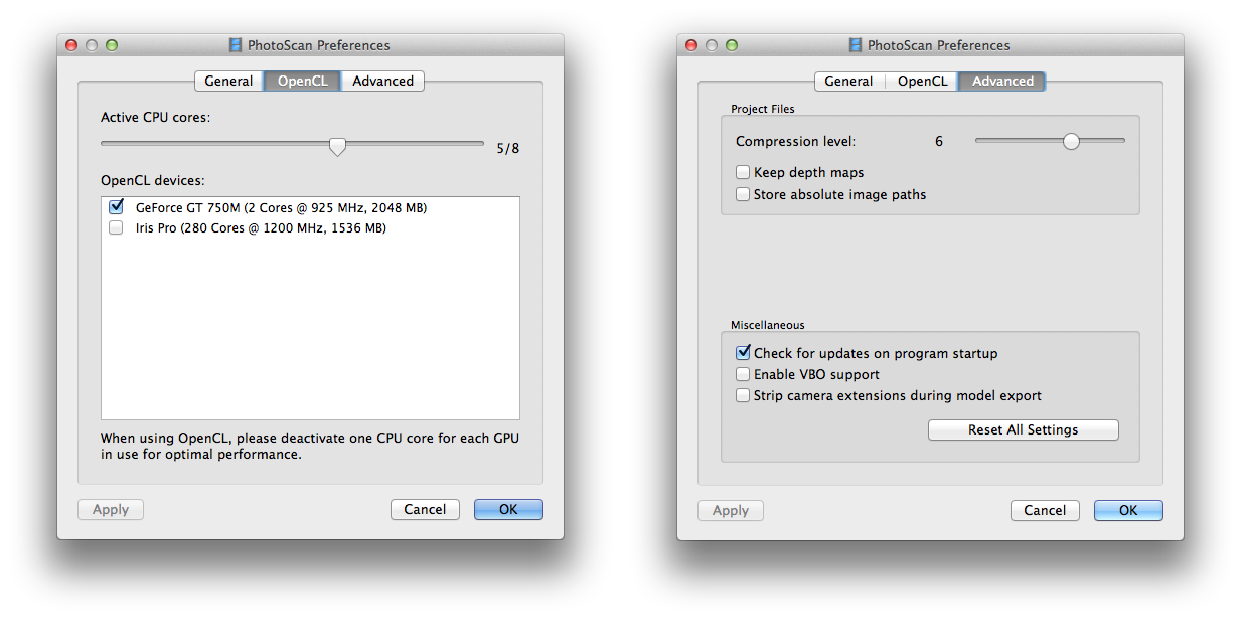
\includegraphics[width=1\textwidth]{PhotoScan-setup}

  \caption{PhotoScan example preference settings}

  \label{fig:photoscansetup}
\end{figure}

Agisoft PhotoScan is able to detect image features, without prior camera calibration or object definition. However it is recommendable to provide a calibration file if available. The calibration can be done via [Tools] $\rightarrow$ [Camera Calibration\dots] If Desired performance of the later reconstruction can be enhanced by using image masks, This increases the likelihood of a successful model reconstruction, but also affects the time consumption, by reducing the feature space. Image masks can be created inside PhotoScan employing framing tools, known from various image-processing applications. As there are a rectangular selection, 'intelligent scissors' (mostly a form of free selection), 'intelligent paint' (also known as 'lasso' selection) and the 'magic wand' (also known as 'magic pen'). In fact these build-in mask creation tools work less efficient than those known from other applications. When using a "green screen" ,it is recommendable to create the masks outside the program and import them later.
Binary masks were coupled after the original images are imported into PhotoScan.

\subsubsection{Import Photos}
\begin{figure}[!h]
  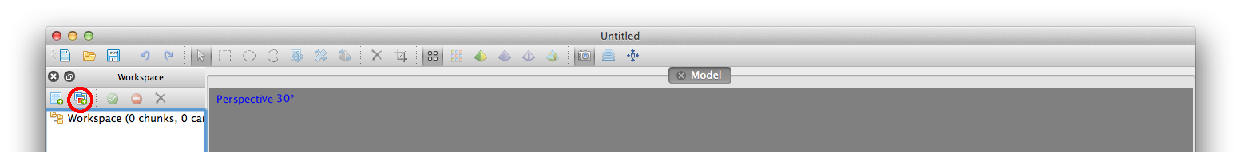
\includegraphics[width=1\textwidth]{PhotoScan-importimages}
  \caption{PhotoScan import images}
    \smallskip
\footnotesize
\begin{changemargin}{0.5cm}{0.5cm}
\centering{The red circle indicates the respective import button.}
\end{changemargin}
  \label{fig:photoscanimpimg}
\end{figure}
Importing pictures can be done by clicking the colored button that was indicated by a red circle in figure~\ref{fig:photoscanimpimg}. After importing all images, the EXIF metadata will be read and used for image alignment if no prior camera calibration took place.
If binary masks are used to define regions of interest, they can be imported via [Tools] $\rightarrow$ [Import] $\rightarrow$ [Import Masks\dots]. Choosing 'From File' will cause an open-dialog to show up in which the folder will be selected where the masks are stored. They will be read according to the name specification prescribed in the editing box. Exemplified the import mask procedure is depicted in figure~\ref{fig:photoscanimpmask}, showing all relevant settings. It is possible to check whether the respective masks were imported correctly, by double clicking one of the thumbnail images located in the lower section of the PhotoScan window, which will display the image with its respective mask overlay.
\begin{figure}[!h]
  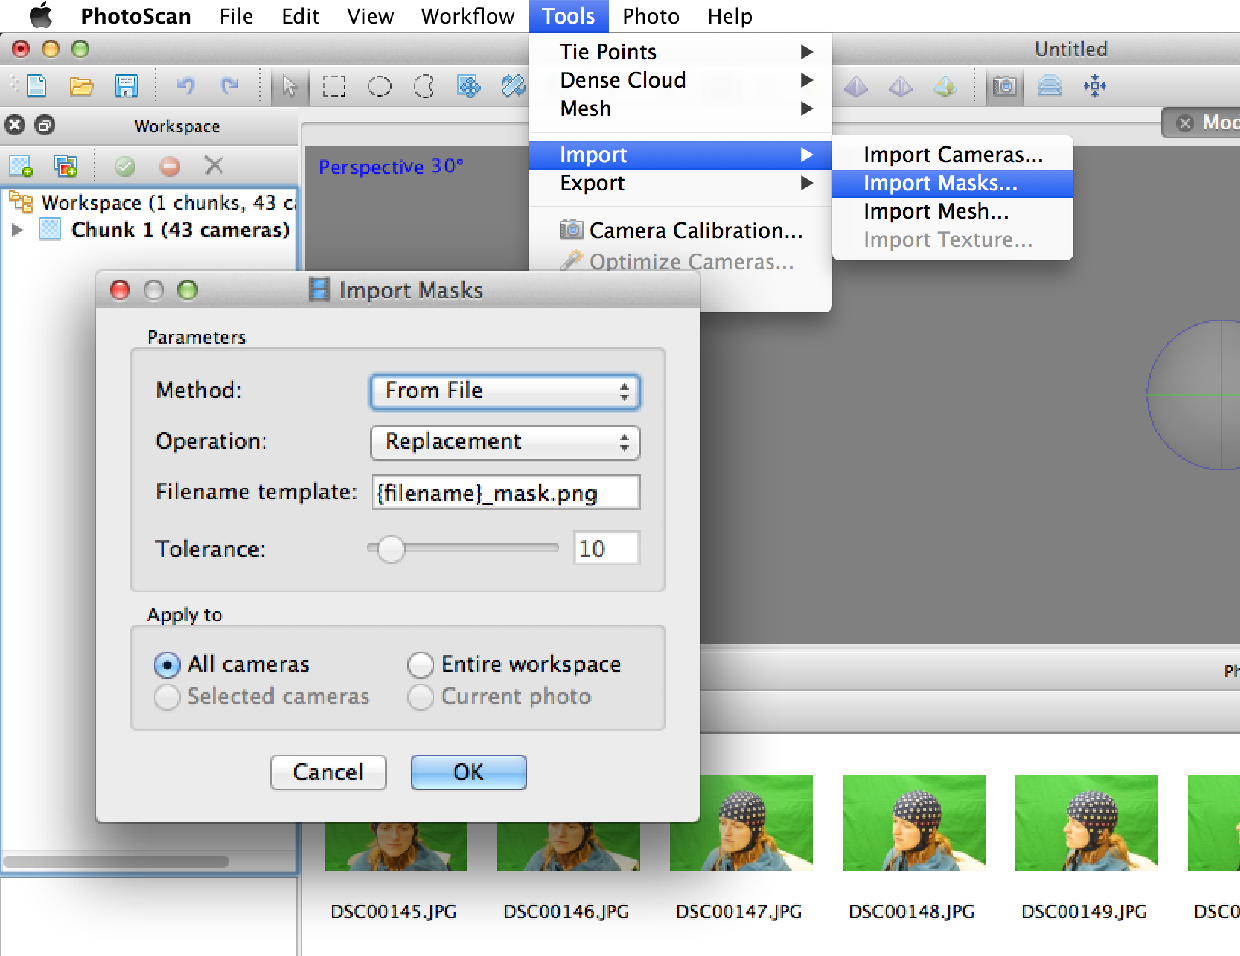
\includegraphics[width=1\textwidth]{PhotoScan-importmasks}
  \caption{PhotoScan import masks}
  \label{fig:photoscanimpmask}
\end{figure}
\FloatBarrier
\subsubsection{Align Photos}
Followed by this procedure, the actual reconstruction can take place. The first step will be to estimate the camera positions based on inherent image features. This can be executed, by selecting [Workflow] $\rightarrow$ [align Photos\dots]. A small setup menu will appear. Actually it remains widely unclear what the exact changes the parameters cause to the processing pipeline, but based on my experience I will give some advices in the following. PhotoScan compares salient image features and tests whether this features match features on another image. If enough features were detected, the camera positions can be estimated. Hence the accuracy value presumably influences the feature detection on the 2D images. An increased accuracy will result in more points that are detected as features yielding a better reconstruction performance. At the same time the processing time and the amount of points that are detected as matching increase, regardless of whether they are. Those false positive points can be limited by selecting a generic 'Pair pre-selection', which reduces the amount of points, based on a certainty measure. At the same time this reduces the processing time tremendously, for what reason I would recommend this option to be set as default. However in some cases (e.g. if image quality is low or too few images were captured), this setting interferes with proper matching point detection and therefore should be disable, in case the first reconstruction attempt failed. Within the 'Advanced' section limitations for the number of points that are going to be detected can be set. Setting those values to 0 will set the limit to infinite. The 'constrain features by mask' option will be available only if masks were imported priorly and does exactly what it is supposed to.
Figure~\ref{fig:photoscanalign}, shows the 'align Photos' step including exemplified settings, depicting also a possible result, that will be called matching point cloud (MPC) from now on.
The next step will be the creation of the dense point cloud (DPC). This step is optional, since the 3D mesh could also be reconstructed employing the MPC, but is crucial for getting high-resolution models.
\begin{figure}[!h]
  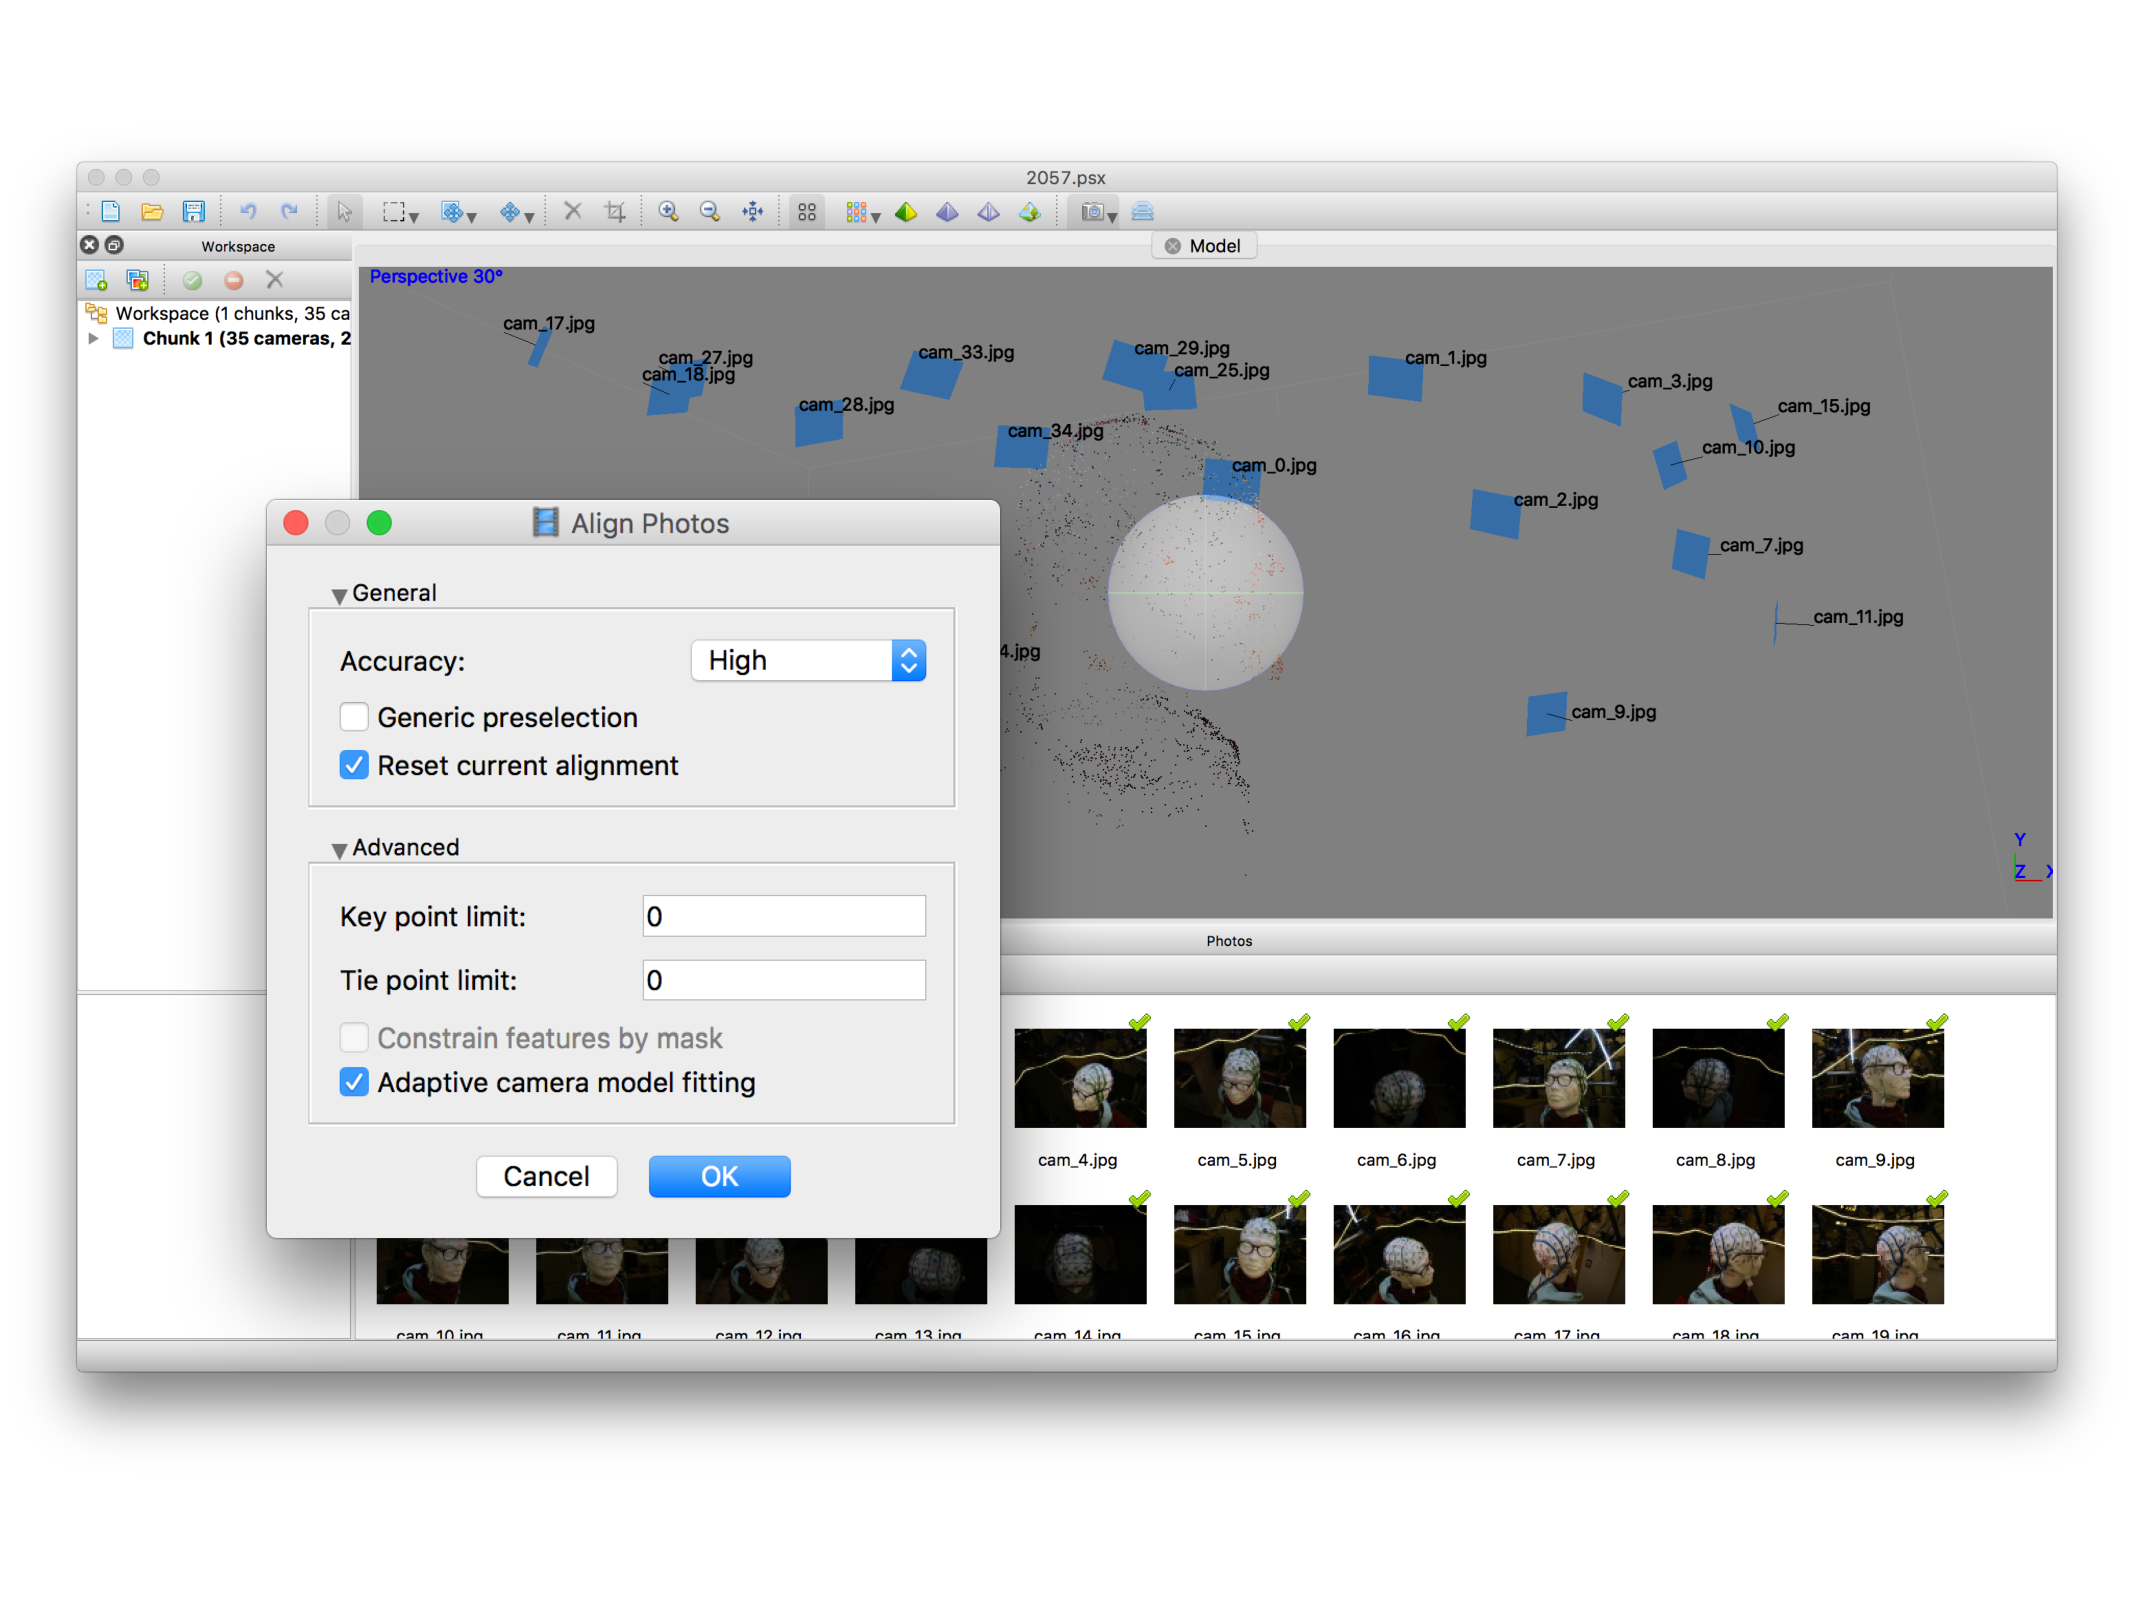
\includegraphics[width=1\textwidth]{PhotoScan-align}
  \caption{PhotoScan align photos}
  \label{fig:photoscanalign}
\end{figure}

\subsubsection{Build Dense Cloud}
PhotoScan uses the basic information of the estimated camera positions, as well as the detected matching points, to reconstruct the depth for image points that lie 'between' the detected features. The final density of the DPC reconstruction depends on the actual resolution of the camera sensor and cannot be compensated by the number of images used.
Figure~\ref{fig:photoscandense} depicts this step including the recommended options. The 'quality' setting affects the density of the final DPC. Setting this to 'High' yields a high-resolution DPC, but keeps the actual processing time relatively short. When this point was set to 'Ultra High' the processing time might increase to several hours, depending on the MPC density, image count and resolution. Within the section 'Advanced' the 'Depth filtering' option can be set. This parameter is used to decide, whether a point is considered as inlier or outlier regarding a reasonable point cloud construction, which therefore affects the smoothness of the DPC. 'Aggressive' depth filtering is recommended, because it keeps the number of irregular mesh extensions on a minimum level.
\begin{figure}[!h]
  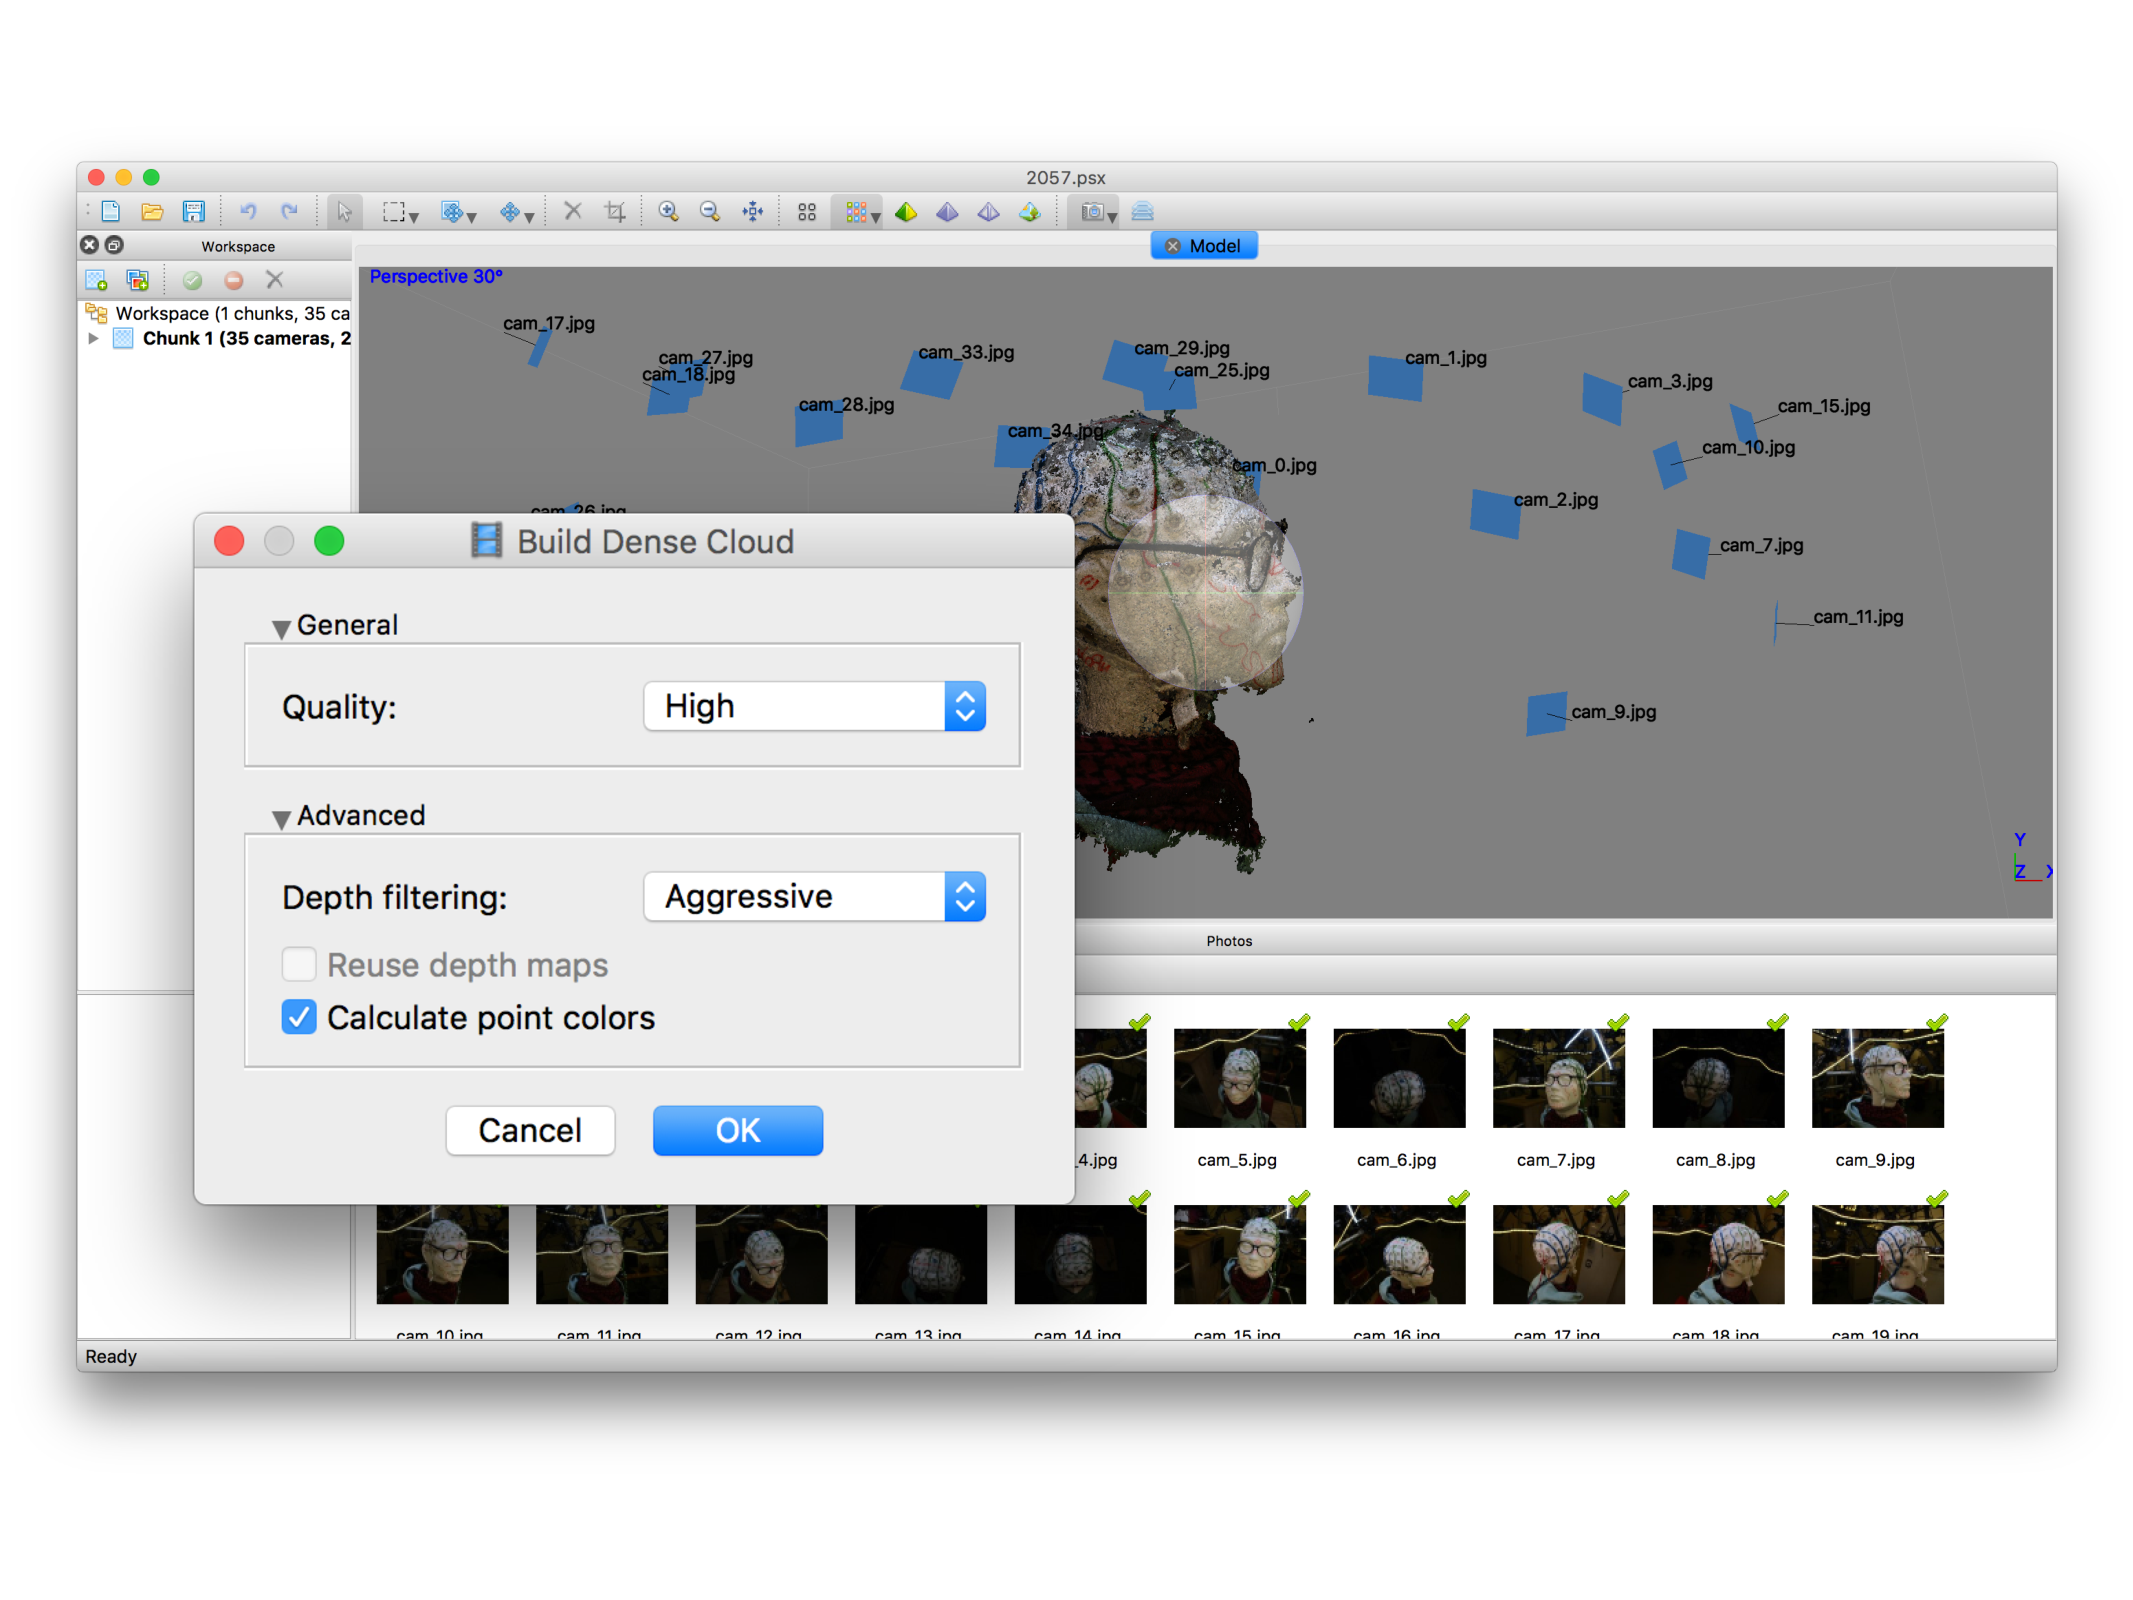
\includegraphics[width=1\textwidth]{PhotoScan-dense}
  \caption{PhotoScan build dense cloud}
  \label{fig:photoscandense}
\end{figure}

\subsubsection{Build Mesh}
As mentioned before, the 3D mesh reconstruction can be based on the MPC or the DPC. Mesh reconstruction in that sense means, that a prior defined point cloud is used as the basis for creating a polygonal triangulated structure. Each face then has a set of 3 corresponding vertex points. Creating the 3D mesh, as shown in figure~\ref{fig:photoscanmesh}, is done by selecting [Workflow] $\rightarrow$ [Build Mesh\dots]. For high-resolution models the source data should be set to 'Dense cloud'. When reconstructing 3D meshes of objects that are not 'relief-like' but instead form a closed 3-dimensional structure (e.g. a human head), the 'Surface type' has to be set to 'Arbitrary'. Because complex meshes like human heads are likely to show lightly uncovered parts on the surface, the vertex point interpolation should be set to 'Enable'.  If the final mesh is used as a 'waterproof' model (e.g. for 3D printing), then it is advisable to set this option to 'Extrapolate', which causes the algorithm to close not only small parts, but instead forcing it to close each part of the mesh.
\begin{figure}[!h]
  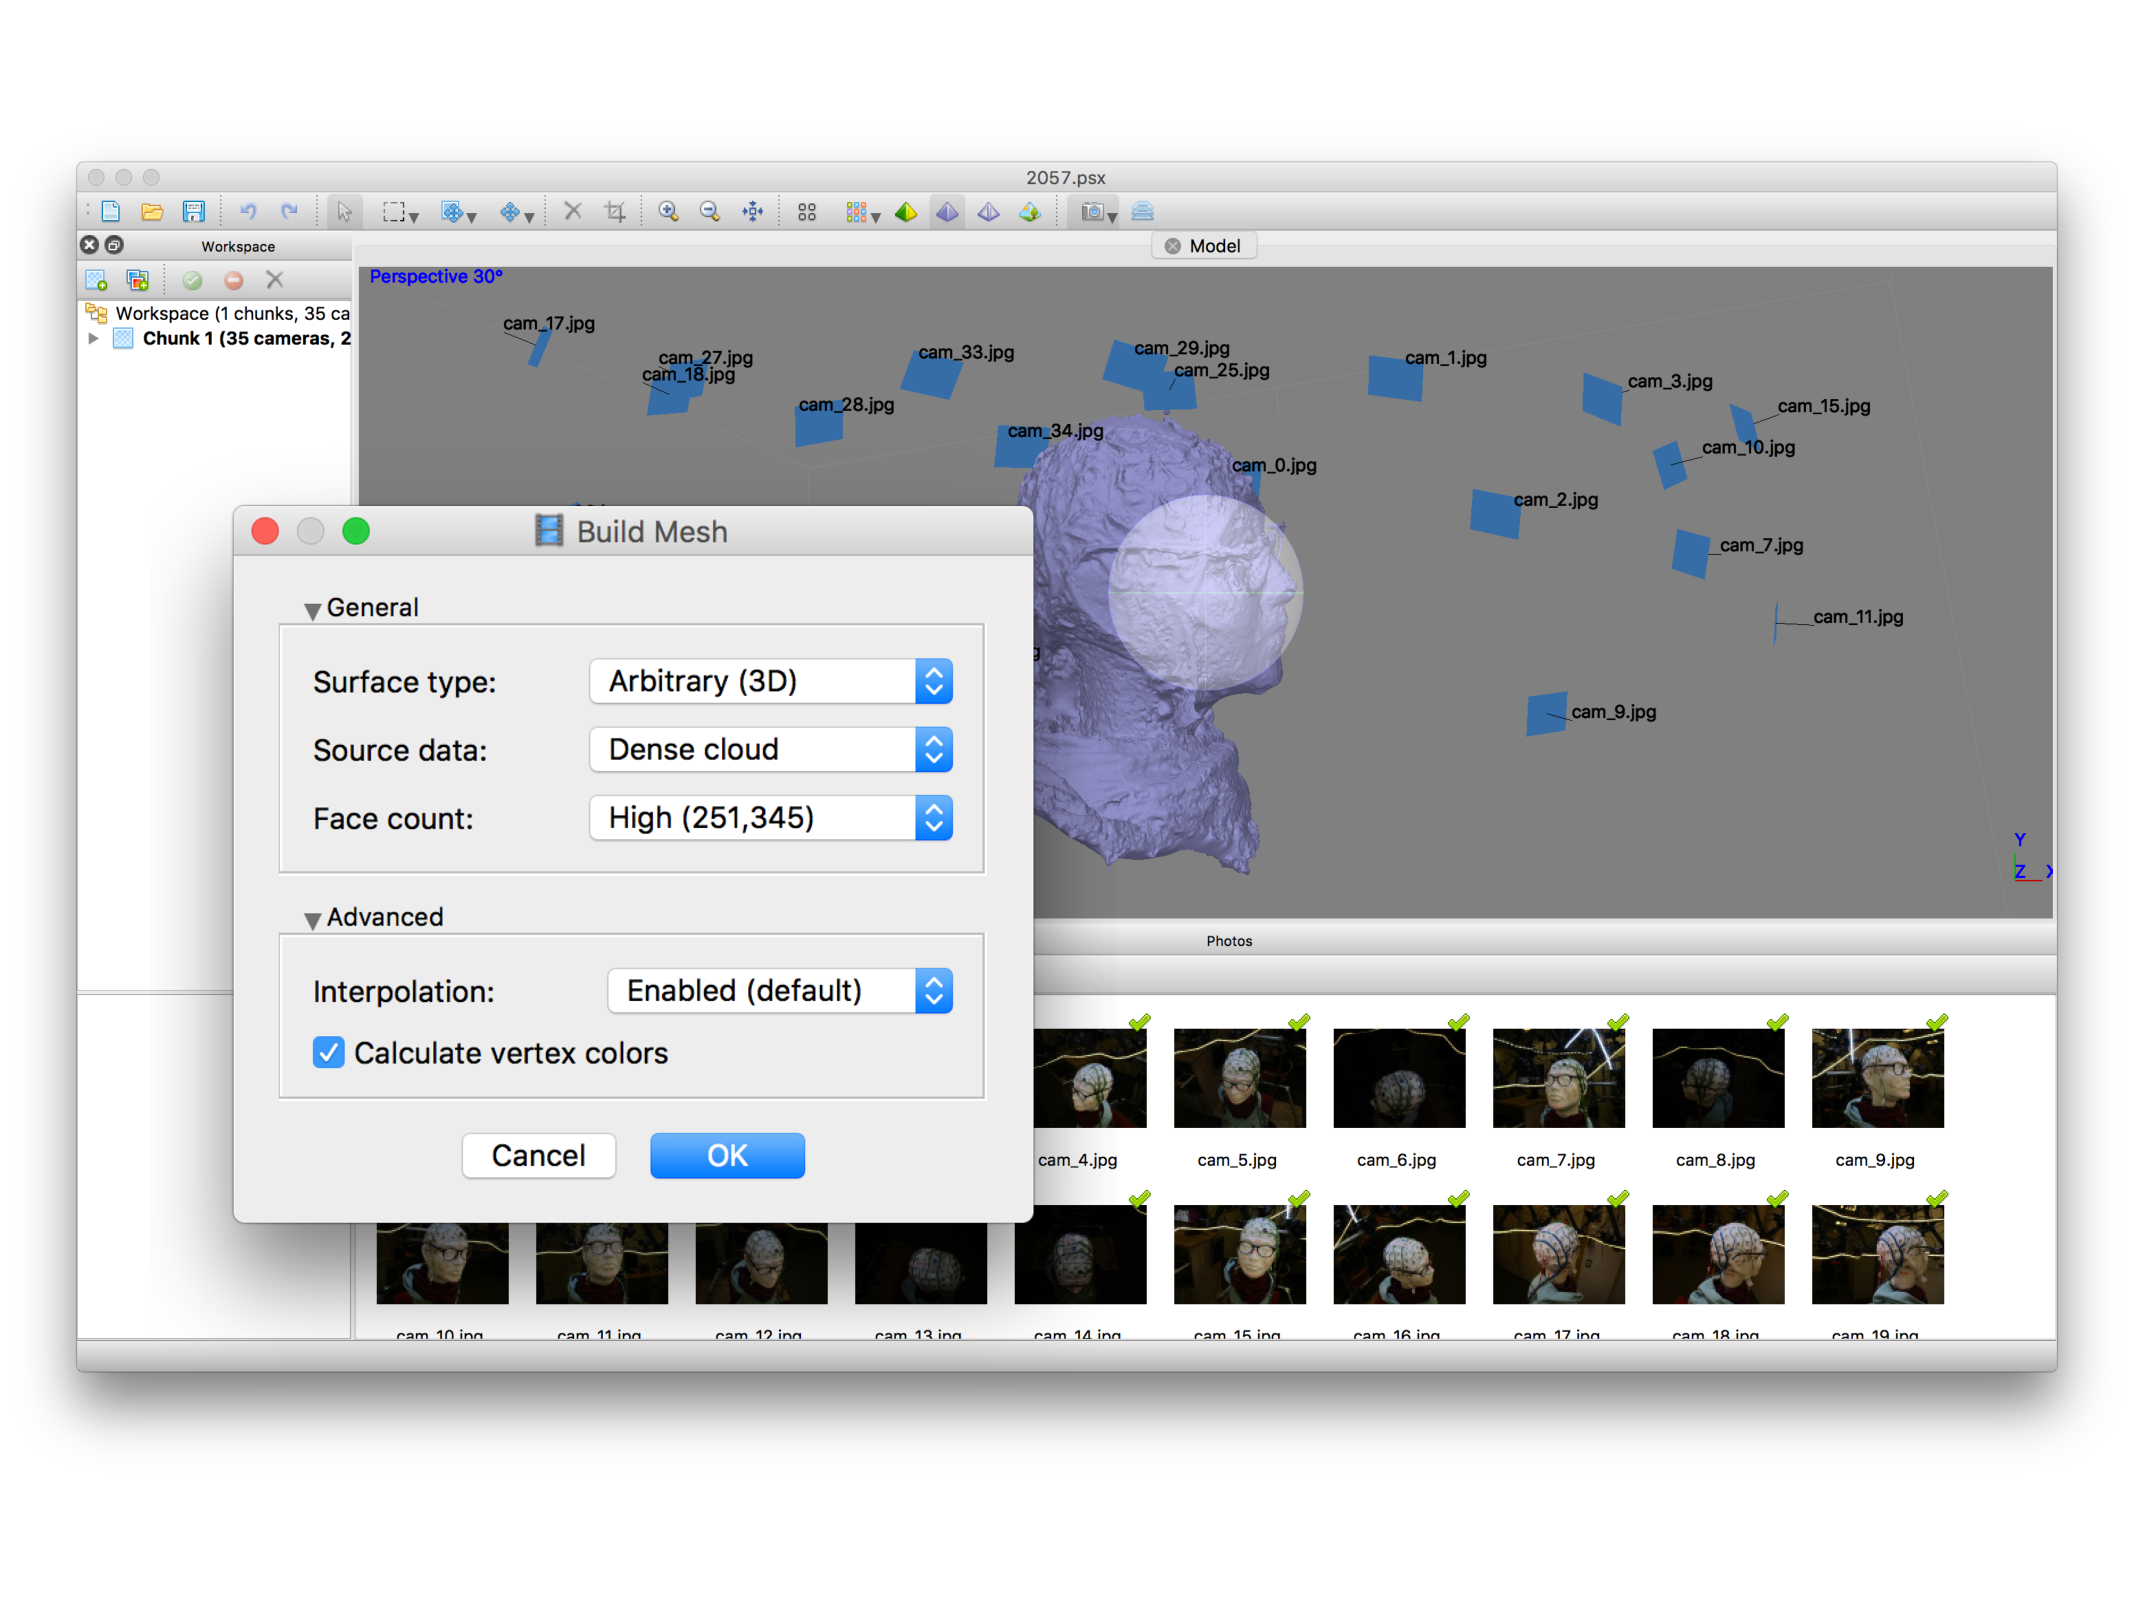
\includegraphics[width=1\textwidth]{PhotoScan-mesh}
  \caption{PhotoScan build mesh}
  \label{fig:photoscanmesh}
\end{figure}
After this step a 3D model out of 2D images was created. Nevertheless it is un-textured so far.

\subsubsection{Build Texture}
Creating the associated texture file can be done by selecting [Workflow] $\rightarrow$ [Build Texture\dots]. Possible settings are shown in figure~\ref{fig:photoscantex}. Depending on the performance of the actual reconstruction those parameters have different influences on the final model. Setting the 'Blending mode' to 'Mosaic' requires all cameras positions to be obtained properly, because it linearly projects color information onto the meshes surface. If one or more camera positions are obtained wrong either smeared or displaced texture parts that overlap the 'true' one can be observed. In that case it is recommendable to set the blending to 'Average', which causes PhotoScan to add the texture by averaging color information of the related camera positions instead of summing them up. Per default the texture file will be split into 25 parts, which, depending on the 3D software used for later processing, can be problematic. For example janus3D can only read one single texture file associated to the model. So when using the textured model as input file for janus3D the texture count should be set to 1.
\begin{figure}[!h]
  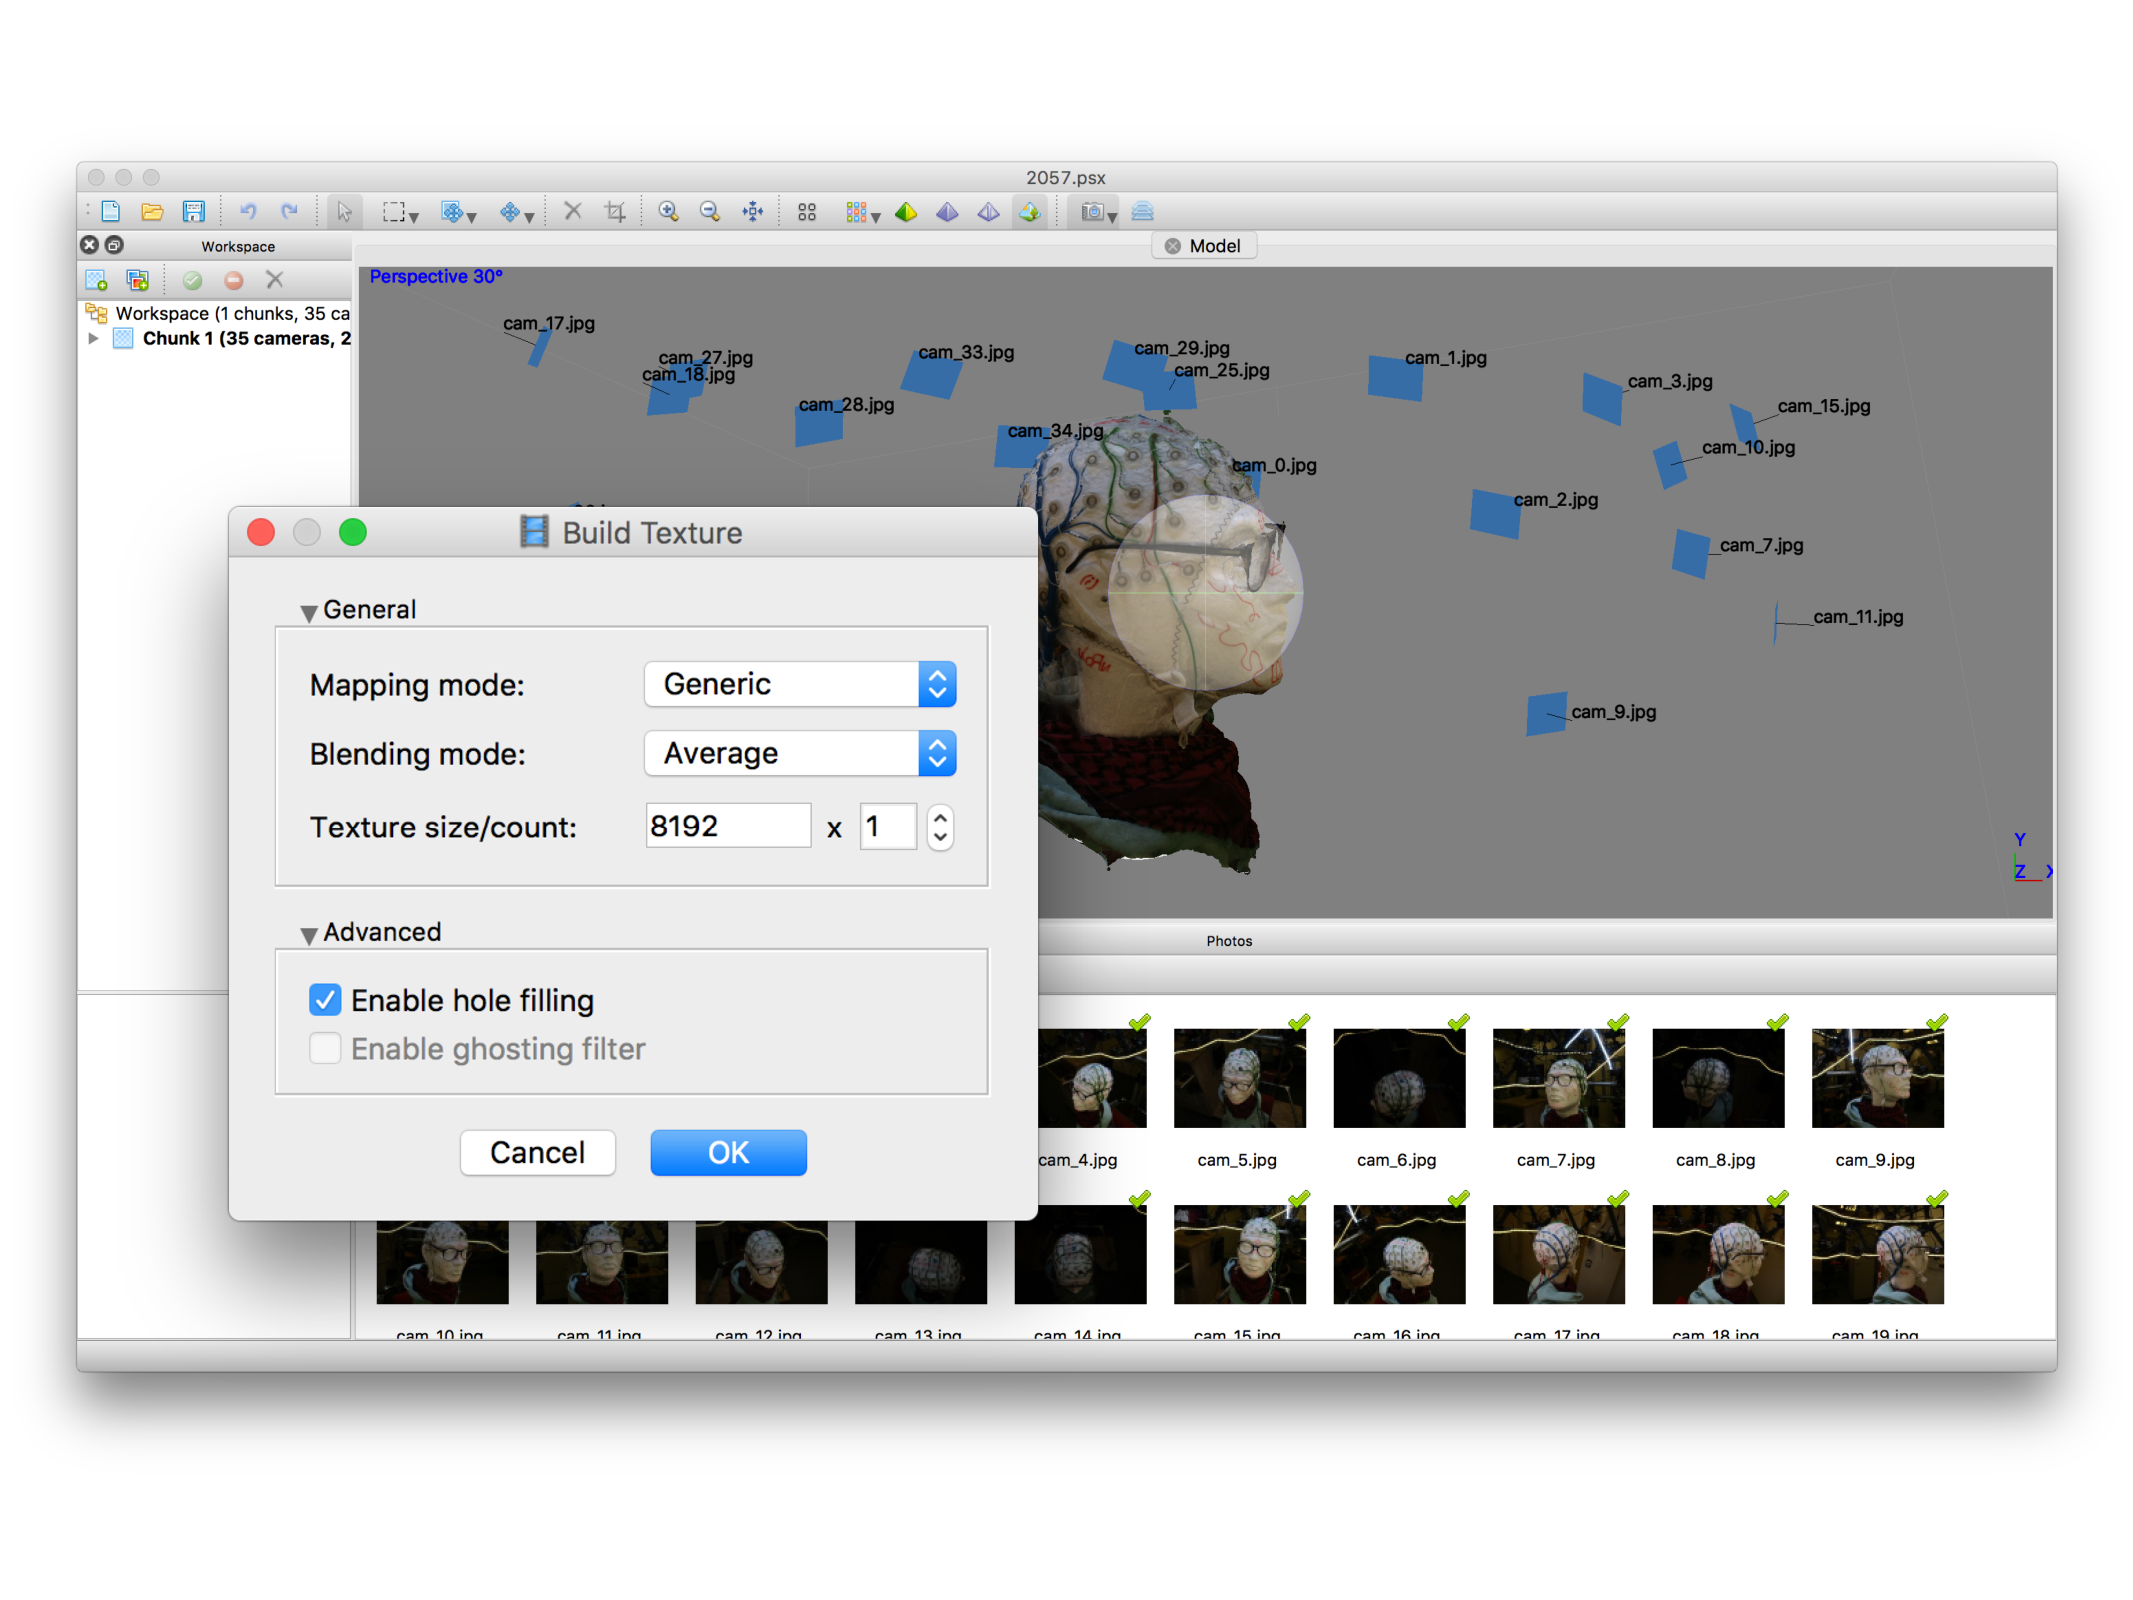
\includegraphics[width=1\textwidth]{PhotoScan-texture}
  \caption{PhotoScan build texture}
  \label{fig:photoscantex}
\end{figure}

\subsubsection{Export Model}
After inspecting the textured model, mesh extensions and parts that will not be used for later processing should be removed. Various selection tools PhotoScan provides can do this. For the purpose of removing mesh extensions the 'free-form selection' yields proper results. The final model can be exported be choosing [File] $\rightarrow$ [Export Model\dots] as shown in figure~\ref{fig:photoscanexport}. Depending on the desired file format export options can vary. Because janus3D can only import objects stored in *.obj (Wavefront OBJ) file format, this was chosen to exemplify this step. It is important to note that for compatibility issues due to the specific requirements of janus3D, only the texture formats *.jpg should be chosen. Furthermore janus3D was not designed to read vertex normals, for what reason this option has to remain unchecked.
\begin{figure}[!h]
  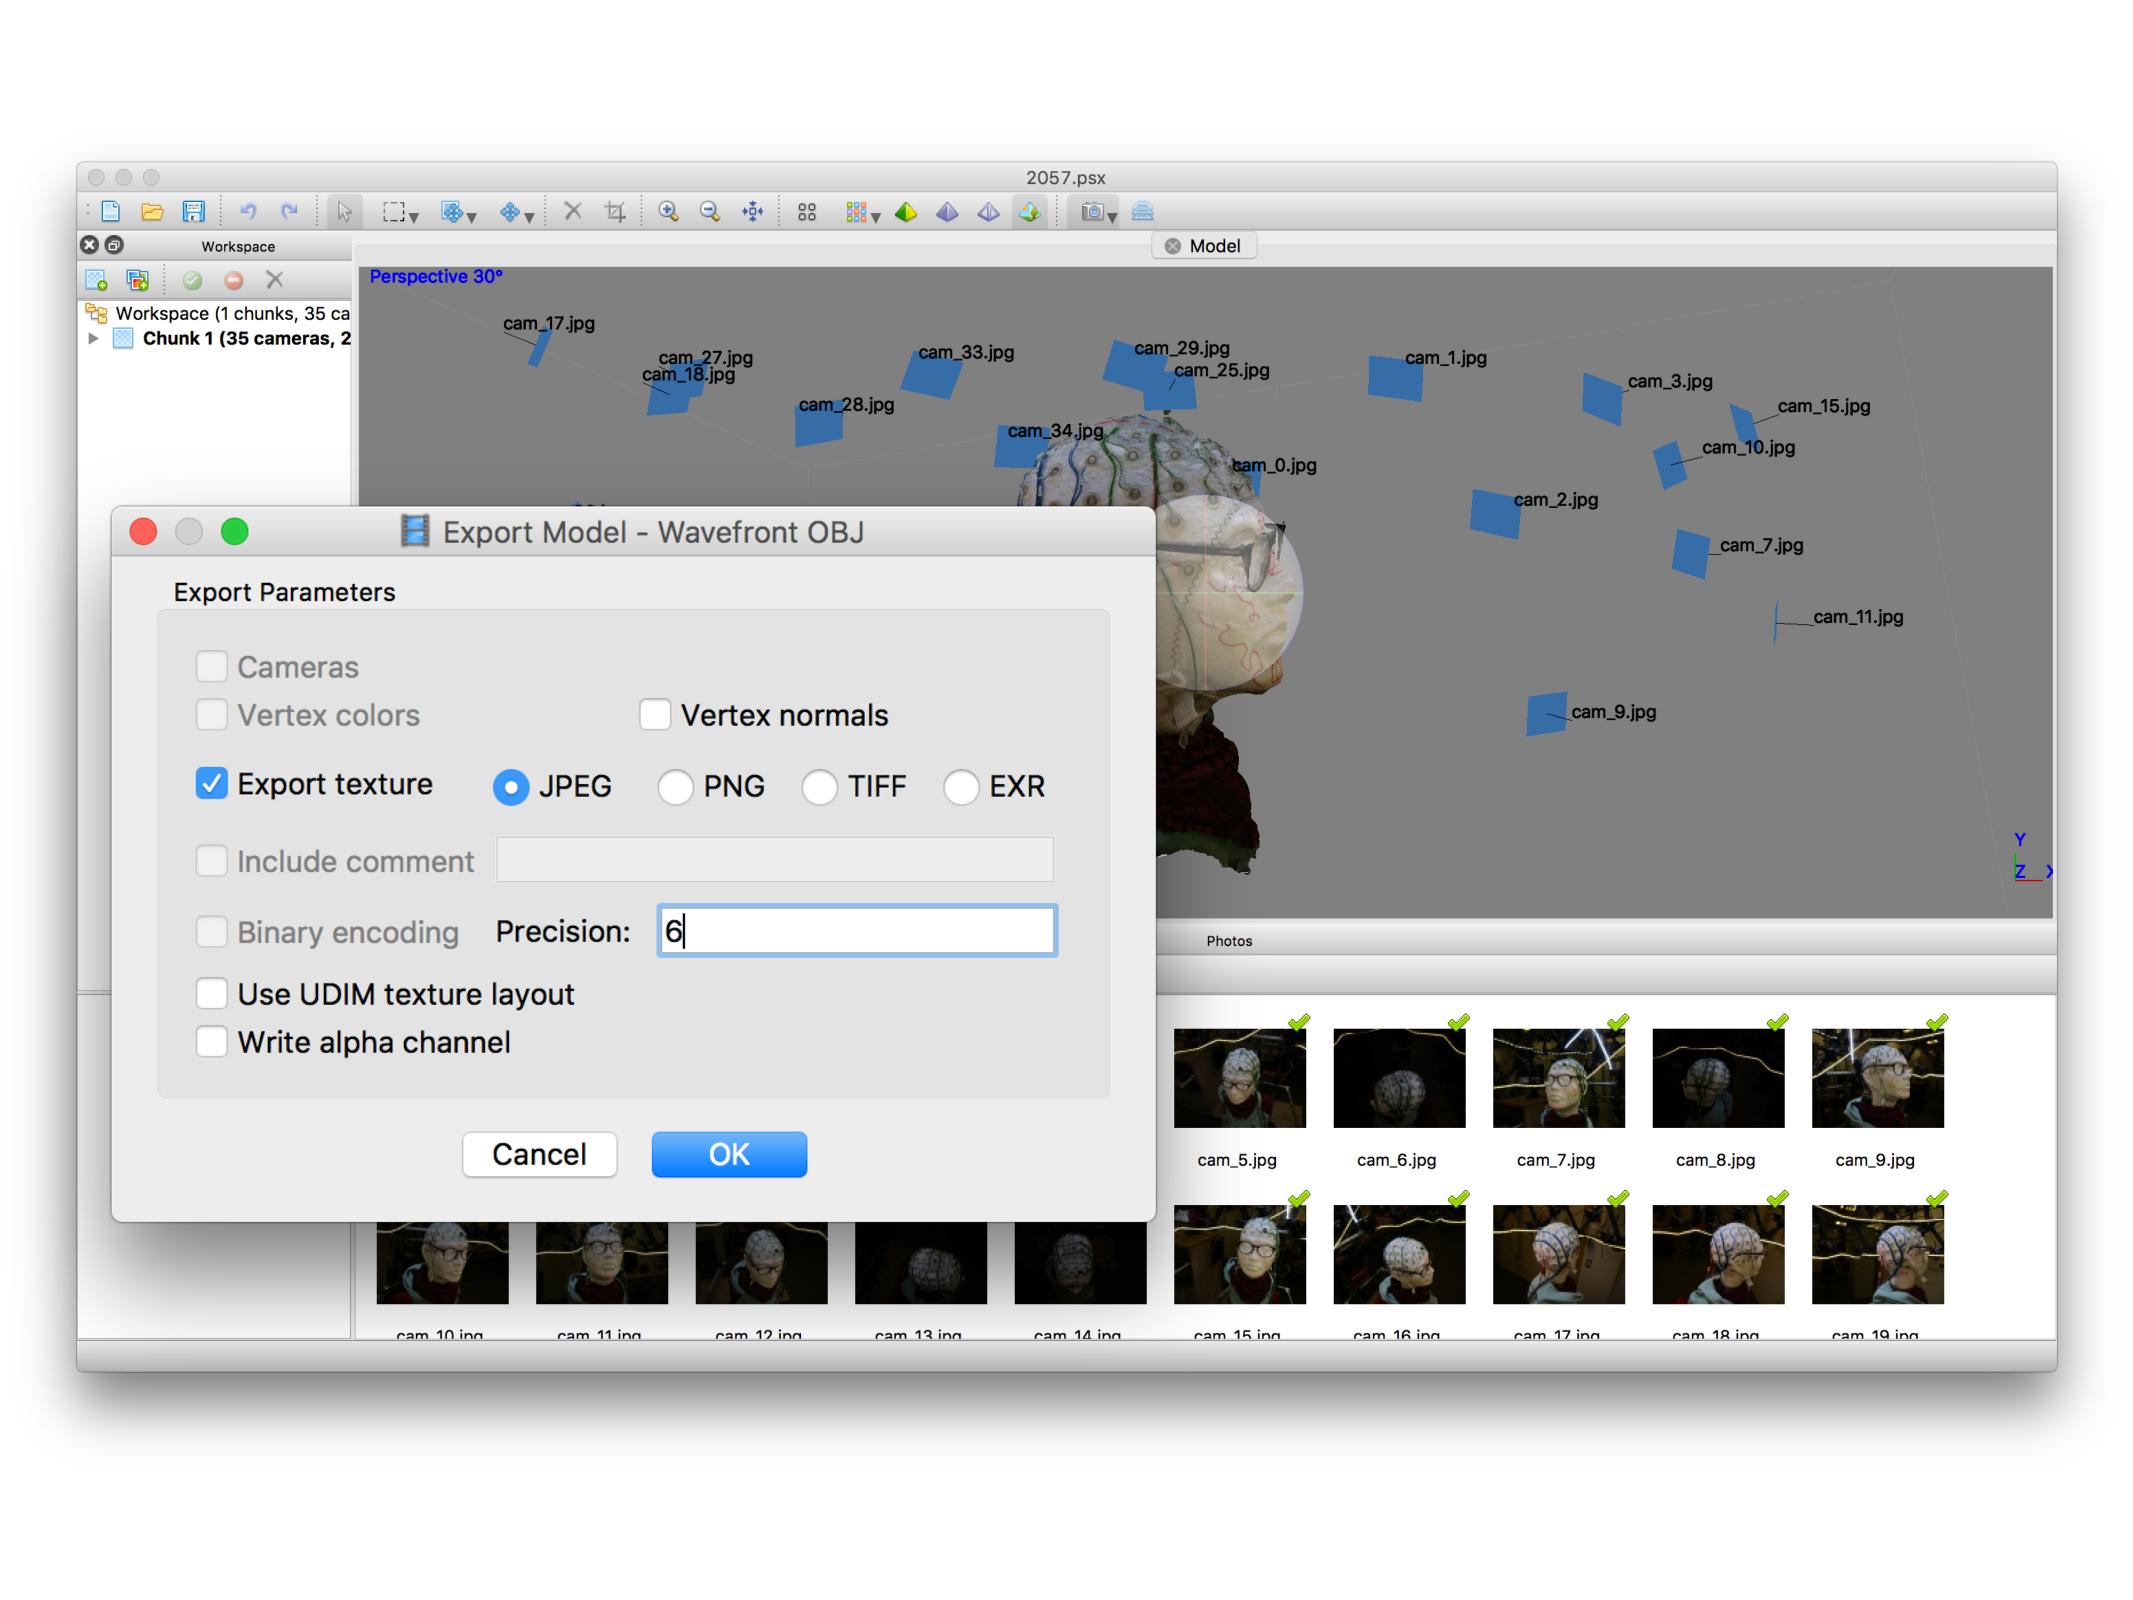
\includegraphics[width=1\textwidth]{PhotoScan-export}
  \caption{PhotoScan export model}
  \label{fig:photoscanexport}
\end{figure}

\FloatBarrier


\subsection{janus3D}
\label{sec:janus3D}
janus3D is a MATLAB toolbox for co-registration and electrode detection and labeling for 3D models obtained from subjects wearing an EEG cap. The software registers the 3D model and a projection of the anatomical MRI, finds electrodes based on the texture or manually, and labels electrodes based on a template or mamually.\\
The toolbox can be downloaded via:\\

\href{https://github.com/janus3D/janus3D_toolbox}{\nolinkurl{https://github.com/janus3D/janus3D_toolbox}} or using the command:\\

\begin{lstlisting}[
    language=Shell,
    basicstyle=\small,
    breaklines=true]
    git clone https://github.com/janus3D/janus3D_toolbox
\end{lstlisting}

Afterwards add the toolbox to the MATLAB search path. One major issue is that the software runs in MatLabR2015a only.\\
Please find the respective information within the janus3D documentation (\href{https://github.com/janus3D/janus3D_toolbox/blob/master/janus3D_users_manual.pdf}{\nolinkurl{https://github.com/janus3D/janus3D_toolbox/blob/master/janus3D_users_manual.pdf}})\\

\noindent After using janus 3D export the set of electrodes to:\\
\begin{center}
  S$<$number$>$/rawData/electrodes/photogrammetry/electrodes.mat
\end{center}

\end{document}
